\chapter{Introduction}
\label{c:introduction}
Scheduling is the coordination layer that keeps factories, transport networks, and data centers productive. Classical methods—priority dispatching rules, tuned metaheuristics, and mixed-integer programming—remain strong benchmarks, yet they struggle when arrivals are stochastic, tariffs and emission factors shift, buffers are finite, or safety and transport constraints couple decisions. Reinforcement learning (RL) promises adaptive dispatch policies that learn from interaction or logs, handle structured state spaces, and react faster than re-optimizing solvers. The recent surge of RL schedulers shows promising gains, but evidence is uneven: many results are single-seed, simulator-bound, and light on feasibility, latency, explainability, or gap-to-optimum reporting. Decision-makers need clarity on when adaptive policies truly dominate and when they simply reshuffle costs or shift risk.

Industrial practitioners ask two pragmatic questions: When does RL decisively outperform mature heuristics or metaheuristics, and how trustworthy are the claims? The daily reality adds layers: tariffs and emission factors change hourly, downtime and rush orders break assumptions, and stakeholders demand latency-budgeted, auditable decisions. This thesis responds with a PRISMA-aligned systematic review of RL for scheduling (2016--2025) across manufacturing and semiconductor flows, logistics/transport dispatch, cloud/edge scheduling, and energy/carbon-aware operations. The review distills design patterns (state/action/reward, masking and shields, hybrids), empirical performance against varied baseline strength, generalization and robustness evidence, and reporting hygiene (seeds, splits, latency, feasibility). It highlights where RL policies hold under disturbances, where hybrids or safety layers are indispensable, and where claims rely on narrow benchmarks.

Recurring themes in the recent RL-for-scheduling corpus include interest drivers—volatile arrivals, richer telemetry, and graph/attention encoders that respect structure—as well as friction points such as long-horizon credit assignment, reproducibility gaps, and safety/feasibility handling. Figure~\ref{fig:intro-scope} maps the scope of the thesis across domains and cross-cutting themes. Throughout, the narrative avoids first-person plural and treats the study as a single-author monograph, keeping emphasis on evidence quality and deployment realism rather than research hype.

\begin{figure}[t]\centering
  \begin{tikzpicture}[
    box/.style={draw, rounded corners, align=center, fill=gray!10, font=\footnotesize, minimum width=4.2cm, minimum height=1.25cm},
    arrow/.style={-Stealth, thick}
  ]
    \node[box] (manu) at (0,0) {Manufacturing\\JSS/FJSS/fabs};
    \node[box] (logi) at (5,0) {Logistics/Transport\\AGV, yards, rail, ride-hailing};
    \node[box] (cloud) at (10,0) {Cloud/Edge\\placement/offloading};
    \node[box] (energy) at (5,2.8) {Energy/Carbon-Aware\\cross-domain};
    \node[box] (themes) at (5,-2.8) {Cross-cutting\\stability, constraints, sim-to-real, safety, reproducibility};

    \draw[arrow] (manu) -- (themes);
    \draw[arrow] (logi) -- (themes);
    \draw[arrow] (cloud) -- (themes);
    \draw[arrow, dashed] (energy) -- (manu);
    \draw[arrow, dashed] (energy) -- (logi);
    \draw[arrow, dashed] (energy) -- (cloud);
  \end{tikzpicture}
  \caption{Scope map of the thesis. Domain chapters feed into cross-cutting themes; energy/carbon-aware objectives intersect all domains.}
  \label{fig:intro-scope}
\end{figure}

\textbf{Research questions}
\begin{itemize}
  \item Where do RL schedulers outperform dispatching rules, metaheuristics, and exact methods, and under which constraints and baselines?
  \item Which design patterns (masking, graph/attention encoders, hybrids) drive stability, feasibility, and generalization across sizes and domains?
  \item How robust are reported gains to seeds, size/domain shifts, tariffs/disturbances, and sim-to-real gaps, including latency and safety claims?
  \item What reporting and benchmarking practices are required for reproducibility and deployment readiness, including offline/shielded evaluation?
\end{itemize}

\textbf{Contributions}
\begin{itemize}
  \item A PRISMA-guided corpus and coding of 60 RL scheduling studies across domains, with quality flags, generalization annotations, and feasibility/latency notes.
  \item A taxonomy of RL method families and design patterns tailored to scheduling, plus comparative performance synthesis by baseline strength (heuristics, metaheuristics, exact).
  \item A cross-cutting challenge analysis (stability, constraint handling, sim-to-real, interpretability/safety, reproducibility) with stress-test and reporting checklists.
  \item A deployment playbook (offline replay $\rightarrow$ shadow $\rightarrow$ shielded limited actuation) and benchmarking blueprint with tariff/disturbance catalogs and offline RL baselines.
  \item A forward-looking roadmap highlighting hybrid RL+OR integration, offline/safe RL for regulated domains, and standardized multi-domain benchmark suites.
\end{itemize}

\textbf{Thesis structure}
\begin{itemize}
  \item \textbf{Chapter~\ref{c:background} Background}: expands scheduling and RL foundations, harmonizes notation, reviews benchmark families, and defines evaluation metrics so later chapters can be read without external references; it also anchors terminology for constraints, buffers, arrival processes, and energy signals.
  \item \textbf{Chapter~\ref{c:methodology} Methodology and PRISMA Protocol}: details the search strategy, databases, time window, inclusion/exclusion criteria, screening flow, quality appraisal rubric, and coding scheme; explains how studies are tagged for baselines, generalization, safety handling, and latency reporting.
  \item \textbf{Chapter~\ref{c:taxonomy} RL Method Taxonomy}: systematizes algorithm families, encoder choices, masking/shielding patterns, reward designs, and hybrid RL+OR integrations; clarifies when to favor value-based, policy-gradient, offline, or model-based approaches under different constraint regimes.
  \item \textbf{Chapter~\ref{c:analysis} Comparative Performance Analysis}: synthesizes empirical evidence against heuristic, metaheuristic, and exact baselines; dissects robustness to seeds, size/domain shifts, tariffs, disturbances, and feasibility under safety layers; reports where RL genuinely closes optimality gaps versus tuned baselines.
  \item \textbf{Chapter~\ref{c:domains} Application Domains}: aggregates domain-specific findings for manufacturing and fabs, logistics/transport, cloud/edge, and energy/carbon-aware scheduling; surfaces stressors such as blocking, headways, SLAs, and tariff windows, and shows how design patterns transfer—or fail—across domains.
  \item \textbf{Chapter~\ref{c:challenges} Cross-cutting Challenges}: examines stability, feasibility/safety enforcement, sim-to-real transfer, interpretability, and reproducibility gaps; proposes mitigation checklists, stress-test catalogs, and reporting templates aligned with deployment expectations.
  \item \textbf{Chapter~\ref{c:future} Open Gaps and Future Directions}: lays out a research agenda and roadmap for robust, deployable RL schedulers, including hybridization opportunities, offline/safe RL trajectories, benchmark suite needs, and verification practices demanded by regulated settings.
  \item \textbf{Chapter~\ref{c:conclusion} Conclusion}: distills a deployment playbook, a reporting checklist, and practitioner guidance that connect the review findings to staged rollout plans, shadow and shielded deployment, and data/latency readiness.
\end{itemize}

\chapter{Background}
\label{c:background}
This chapter establishes a common vocabulary before the detailed synthesis that follows. It spans three pillars: (i) the scheduling problem classes and constraints encountered in the RL literature; (ii) the RL building blocks most frequently adapted to scheduling; and (iii) the benchmarks, metrics, and baselines that shape how evidence is reported. The goal is a self-contained primer that lets readers parse the later chapters without having to infer definitions or assumptions.

\section{Scheduling Fundamentals}
Scheduling problems vary along routing freedom, machine parallelism, buffer assumptions, and whether arrivals are known upfront. Table~\ref{tab:scheduling-archetypes} summarizes canonical classes and the design implications for RL agents; the accompanying text keeps terminology consistent without relying on an illustration.

Classical job shops (JSS) assume fixed operation sequences and single machines, while flexible job shops (FJSS) add routing choices that expand the action space. Flow shops (and hybrid flow shops) introduce stage-wise flow with parallel machines per stage and often blocking/no-wait constraints. Parallel-machine and batching problems center on grouping tasks while managing setups and release dates. Dynamic variants inject arrivals, processing-time noise, and downtime; transport problems (AGVs, cranes, truck dispatch) couple routing with safety constraints like headways or charging windows. Cloud and edge scheduling resembles parallel machines with network and SLA constraints.

Constraints fall into three categories. \textit{Hard constraints} (precedence, machine capacity, headways, safety zones) cannot be violated; RL agents typically enforce them via action masks or shields. \textit{Soft constraints} (due dates, penalties for lateness, desired energy budgets) are usually encoded as reward terms or Lagrangian penalties. \textit{Operational policies} (setup batching, buffer limits, maintenance calendars) sit in between: they may be enforced through mask logic, reward shaping, or a mixture of both. Many papers implicitly assume infinite buffers, no transport time, and perfect machine availability; when these assumptions change, the observation space and mask logic must change with them.

Dynamic settings require rolling-horizon decision-making. Agents observe a snapshot (queues, remaining routes, machine status) and pick an action that remains fixed over a control interval. Time-discretization is often abstracted: simulators advance to the next event (job finishes, arrival, setup completion), not every second. Explicitly aligning simulator events and policy steps is crucial when comparing wall-clock runtime to heuristics.

State representation choices strongly affect learnability. Minimalistic vectors (queue lengths, remaining time) keep models light but miss graph structure; disjunctive-graph encodings capture precedence and machine conflicts at higher compute cost. Including temporal features (slack, remaining processing, release times) improves tardiness handling; incorporating energy prices or tariffs enables multi-objective trade-offs. Transport problems often need occupancy grids or pairwise distance matrices to enforce collision avoidance. Observation noise is rarely modeled but matters in reality; masking logic must remain correct under noisy or delayed sensors.

Action spaces follow the constraint structure. In static JSS, a single discrete action that selects the next operation suffices. In FJSS, actions often factor into (job, machine) pairs or routing decisions, sometimes combined with a “do nothing”/wait action to allow idle time when tariffs peak. Transport problems add path choices or micro-movements; cloud/edge schedulers add admission/rejection decisions. Poorly designed action spaces explode combinatorially or hide feasible moves; masks or hierarchical decompositions prevent the agent from exploring invalid branches.

Constraint satisfaction is easier when constraints are explicit and testable. Feasibility checkers (unit tests on toy instances) expose stale masks, incorrect precedence handling, or timezone/clock drift in time-indexed problems. Hybrid RL+OR approaches sometimes delegate feasibility to a repair operator; in those cases, the repair cost must be accounted for in the reward to avoid “reward hacking.” Even under perfect masks, simulators must model realistic changeovers (setup times, transport, maintenance) to avoid optimistic results.

\begin{table}[t]\centering\small
  \caption{Scheduling archetypes and RL implications.}
  \label{tab:scheduling-archetypes}
  \begin{tabular}{p{2.6cm}p{3.7cm}p{3.7cm}p{4cm}}
\toprule
\textbf{Problem class} & \textbf{Typical assumptions} & \textbf{Common constraints} & \textbf{RL design implications} \\
\midrule
Job Shop (JSS) & Fixed routing, unit machines & Precedence, machine capacity, due dates & Disjunctive-graph state, masking for machine availability and precedence \\
Flexible Job Shop (FJSS) & Alternative machines per operation & Routing choice, setups, re-entrance & Joint routing/dispatch actions; masks couple routing with feasibility; graph encoders \\
Flow/Hybrid Flow Shop & Stage-wise flow, parallel machines per stage & Blocking/no-wait, buffers, sequence-dependent setups & Stage-wise masking; idle/hold actions; penalty terms for blocking \\
Parallel/Batch Machines & Identical/unrelated machines, batching allowed & Batch size, family setups, release dates & Batch-construction action spaces; reward terms for batch balance vs.\ tardiness \\
Dynamic/Online & Job arrivals, stochastic times & Rolling horizon, response-time SLAs & Recurrent/attention states; warm-started value functions; disturbance-aware masking \\
Transport/AGV & Coupled routing and processing & Collision/zone safety, charging windows & Multi-agent or joint action spaces; safety shields for headway/charge \\
Cloud/Edge Scheduling & VM/edge nodes, network latency & SLA/latency, energy caps, affinity & Compact queue states; admission control in action space; power-aware rewards \\
\bottomrule
\end{tabular}

\end{table}

\section{Reinforcement Learning Essentials}
Scheduling papers mostly rely on standard Markov Decision Process (MDP) notation: states capture queues, machine status, elapsed time, and sometimes energy or tariff signals; actions select the next operation/machine pair, a dispatching priority, or (in transport/cloud) a route or placement decision; rewards penalize tardiness, idle time, or energy while rewarding throughput. Few papers deviate from the episodic undiscounted setting, but discount factors are retained to stabilize advantage estimates.

Value-based methods (DQN, DDQN, dueling, distributional variants) remain common for discrete dispatch spaces, especially when action masking keeps Q-values well-behaved. Actor-critic and policy-gradient methods (A2C/A3C, PPO, SAC) dominate recent flexible shops and transport work because they scale to large and structured action spaces with GNN encoders. Deterministic policy gradients (DDPG/TD3) appear when actions are continuous (setpoints, timing, continuous resource allocation). Model-based and Dyna-style schemes are rarer but attractive when simulators are expensive or logs are plentiful. Offline RL is starting to be explored for cloud/edge and for shadow-deployment data.

Exploration must respect feasibility. $\epsilon$-greedy sampling over masked actions and entropy-regularized policies are standard; curricula (simple to complex instances) help stabilize early learning in combinatorial spaces. Replay buffers often separate small and large instances to avoid non-stationary targets. Reward scaling is critical when mixing makespan, tardiness, and energy; several studies normalize by job count or baseline heuristic performance to keep gradients stable. Table~\ref{tab:rl-cheatsheet} distills which algorithm families are suited to which problem traits.

Credit assignment is especially challenging with long horizons and sparse rewards. Advantage normalization, generalized advantage estimation, and value clipping (PPO) appear frequently. Some works shape rewards with stepwise tardiness or idle-time penalties so that signals arrive at every decision, but ablations are rare. When the action space is factored (e.g., choose job then machine), either hierarchical policies or factorized Q-networks can ease learning; both require careful coordination to avoid deadlocks.

Architectural trends mirror the structure of scheduling problems. GNNs over disjunctive graphs excel at variable-size instances; attention layers help the policy focus on critical operations (near due dates, bottleneck machines). CNNs over timetable grids are rare but appear in flow shops; RNNs capture temporal patterns in arrival processes for cloud traces. Multi-agent settings (AGVs, ride-hailing) either centralize training with decentralized execution (CTDE) or use shared critics; collision safety is usually handled by shared masks. Offline and batch RL approaches are promising when logs are abundant but simulators are weak; conservative Q-learning or behavior-regularized objectives can reduce extrapolation error.

Hyperparameter choices dominate stability. Learning rates, entropy coefficients, GAE $\lambda$, and PPO clip ranges interact with mask entropy and reward scaling. Curriculum schedules (instance size, arrival rates) benefit from simple hand-crafted progressions; automatic curricula are still uncommon. Replay buffer hygiene matters: mixing trajectories across scales can destabilize targets, while segregating buffers by difficulty can smooth training. Model persistence (checkpointing seeds, evaluator scripts) is vital for reproducibility but rarely described.

Multi-objective formulations appear in energy-aware and SLA-aware work. Scalarization with weighted sums is the norm; a few studies use lexicographic sorting (feasibility first, then KPI) or Lagrangian multipliers that adapt weights during training. Reporting the weight schedule and sensitivity curves is essential to understand whether gains come from better trade-offs or weight tuning. Pareto front approximations are rare but valuable, especially for stakeholders who must choose between throughput and energy.

Table~\ref{tab:mdp-notation} recaps notation used throughout the thesis. The RL-for-scheduling loop is described textually, emphasizing mask/shield enforcement, logging, and event-driven simulation.

\begin{table}[t]\centering\small
  \caption{RL algorithm families and when to use them for scheduling.}
  \label{tab:rl-cheatsheet}
  \begin{tabular}{p{2.4cm}p{3.2cm}p{3.6cm}p{3.8cm}}
\toprule
\textbf{Family} & \textbf{Strengths for scheduling} & \textbf{Typical pitfalls} & \textbf{When to prefer} \\
\midrule
DQN/DDQN/Dueling & Simple, stable on small discrete spaces; easy masking & Overestimation, slow with huge action sets & Small JSS, baseline dispatchers, ablations \\
Rainbow/Distributional & Better value estimates, handles stochastic rewards & More hyperparameters, variance & Dynamic arrivals with noisy processing times \\
A2C/A3C & Parallelizable, lighter footprint & Higher variance than PPO/SAC & Low-latency online dispatch on embedded hardware \\
PPO (clip/penalty) & Robust to hyperparameters; works well with GNNs & Entropy/mask interaction; reward scaling sensitive & General-purpose JSS/FJSS with medium/large actions \\
SAC (discrete/continuous) & Sample-efficient, entropy-regularized & Temperature tuning; slower inference & Energy-aware problems needing balanced exploration \\
Deterministic PG/DDPG/TD3 & Works with continuous actions (e.g., timings) & Action bounds, exploration noise brittle & Hybrid control with continuous setpoints or durations \\
Hierarchical RL & Decouples routing/dispatch; improves exploration & Credit assignment, more design choices & Large FJSS, transport with joint routing + timing \\
Model-based/Dyna & Data-efficient, supports lookahead & Model errors; higher engineering effort & Expensive simulators, low data budgets, offline priors \\
Offline/Batch RL & Uses logs; safer for regulated settings & Distribution shift; needs conservative Q & Sites without sim access; shadow deployment logs \\
\bottomrule
\end{tabular}

\end{table}

\begin{table}[t]\centering\small
  \caption{MDP notation used in RL-based scheduling.}
  \label{tab:mdp-notation}
  \begin{tabular}{p{2cm}p{4.2cm}p{5.8cm}}
\toprule
\textbf{Symbol} & \textbf{Meaning} & \textbf{Scheduling instantiation} \\
\midrule
$s_t$ & State at decision step $t$ & Queues, machine status, remaining routes, clock time, energy price, backlog \\
$a_t$ & Action at step $t$ & Pick operation-machine pair; choose route; assign job to VM/edge node; dispatch vehicle \\
$\mathcal{A}(s_t)$ & Feasible action set & Masked legal moves obeying precedence, capacity, safety, or SLA rules \\
$r_t$ & Reward & Negative makespan/tardiness increment, energy cost, SLA penalty, or composite \\
$\gamma$ & Discount factor & Usually in $[0.9, 1.0]$; often close to $1$ for long-horizon scheduling \\
$P(s_{t+1}\mid s_t,a_t)$ & Transition dynamics & Simulator of processing, travel, setups, arrivals; may include stochasticity \\
$\pi_\theta(a\mid s)$ & Policy & Neural dispatcher (MLP, CNN, GNN, attention) producing masked logits or scores \\
$V_\phi(s)$ & Value function & Baseline/critic estimating downstream cost; often shared encoder with policy \\
$\hat{J}(\pi)$ & Objective & Expected cumulative reward or multi-objective scalarization (makespan/energy) \\
\bottomrule
\end{tabular}

\end{table}

\section{Benchmarks and Metrics}
Evidence quality depends on benchmark selection, metric reporting, and the strength of baselines. Most manufacturing work still leans on FT/LA/Taillard splits; flexible shops use BRdata; dynamic shops rely on bespoke generators. Transport studies design proprietary layouts; cloud papers mix synthetic and public traces; port/yard studies sometimes publish logs but not simulators. Table~\ref{tab:benchmark-suites} summarizes commonly used suites and what they probe. A PRISMA-style summary of the literature matrix is in Chapter~\ref{c:methodology}; here the emphasis is on why particular benchmarks matter for evaluating RL policies.

Metrics must capture both optimality and feasibility. Makespan and tardiness remain primary; energy/carbon metrics appear in sustainability-focused work; SLA violations, percentile latencies, and utilization are central to cloud/edge studies; safety violations matter in AGV/rail settings. Table~\ref{tab:metrics-glossary} gives short definitions and notes on how to report them credibly. Figure~\ref{fig:metric-emphasis} visualizes how often these metrics appear across domains (qualitative scores from the surveyed corpus).

Baselines anchor claims: priority dispatching rules (SPT, EDD, LPT) set a minimal bar; tuned metaheuristics (GA, SA, TS, PSO, hybrids) represent practitioner-strength baselines; MILP/CP provide optimality gaps on small instances; simple bin-packing heuristics are essential in cloud/edge. Reporting should also include decision latency of both RL and baselines, since real systems operate under control-cycle deadlines.

For meaningful comparisons, studies should publish train/validation/test splits and avoid tuning on test instances. Stress suites (arrival bursts, tariff shifts, downtime injections) reveal brittleness. Whenever possible, per-instance results should accompany averages so that variance and tail failures are visible. Many static-benchmark results overstate generalization; dynamic or multi-seed evaluations narrow this gap.

Reproducibility requires open assets: generators for synthetic instances, disturbance and tariff catalogs, and scripts that recompute all KPIs from logged trajectories. When proprietary data prevent release, papers should disclose summary statistics (size distributions, routing depth, variance of processing times) and still report on public benchmarks. Seeds, hardware, and wall-clock runtimes should accompany every table or plot. Confidence intervals or standard deviations across seeds are preferred over single best-seed numbers. Without these basics, later chapters’ calls for standard protocols cannot be acted on.

\begin{table}[t]\centering\small
  \caption{Benchmark suites appearing in RL scheduling studies.}
  \label{tab:benchmark-suites}
  \begin{tabular}{p{3cm}p{3.5cm}p{3.2cm}p{3.8cm}}
\toprule
\textbf{Suite / source} & \textbf{Scale / features} & \textbf{What it probes} & \textbf{RL usage notes} \\
\midrule
FT06/10/20, LA & Small--medium JSS & Dispatch quality, makespan gap to optimum & Masks guarantee feasibility; useful for ablations and gap-to-optimum reporting \\
Taillard (tai20--100) & Medium--large JSS/FJSS & Cross-size generalization, scalability & Popular for train/val/test splits; supports curriculum from small to large \\
BRdata / OR-Lib & FJSS with alternate machines & Routing/dispatch coupling & Good for testing routing masks and dual-attention encoders \\
Dynamic JSS generators & Arrival bursts, stochastic times & Robustness to non-stationarity & Enables stress suites with downtime and rush orders \\
AGV/warehouse layouts (bespoke) & Multi-AGV, collisions, charging & Safety and multi-agent coordination & Requires shields/masks; latency constraints matter \\
Port/yard traces & Trucks, cranes, energy tariffs & Sim-to-real signal quality & Real traces for domain randomization; compare to rule-based dispatch \\
Cloud traces (Google, Alibaba) & Heterogeneous jobs, deadlines & SLA, energy bins, resource fragmentation & Supports batch/offline RL; admission and bin packing baselines needed \\
Edge/IoT toy suites & Small graphs, limited compute & Decision latency under constraints & Useful for profiling policy runtime vs.\ heuristics \\
\bottomrule
\end{tabular}

\end{table}

\begin{table}[t]\centering\small
  \caption{Metrics and KPIs with reporting notes.}
  \label{tab:metrics-glossary}
  \begin{tabular}{p{2.6cm}p{3.8cm}p{6cm}}
\toprule
\textbf{Metric / KPI} & \textbf{Definition (informal)} & \textbf{Notes for RL evaluation} \\
\midrule
Makespan $C_{\max}$ & Completion time of last job & Report gap to optimum/MILP where available; include decision latency if inference is non-negligible \\
Total/mean tardiness & Sum/mean of delays beyond due dates & Distinguish lateness vs.\ tardiness; show distribution, not just mean \\
Flow time / WIP & Time jobs spend in system; work-in-process & Sensitive to dispatch jitter; useful for dynamic shops and queues \\
Energy / carbon & kWh or kg CO$_2$e consumed & Specify tariff, PUE, emission factors; report trade-offs vs.\ throughput \\
SLA violation rate & Fraction of jobs exceeding deadlines & Standard in cloud/edge; pair with tail latency (p95/p99) \\
Throughput & Jobs completed per unit time & For transport/AGV and cloud workloads; pair with utilization \\
Utilization / busy ratio & Fraction of resource busy time & Helps interpret makespan improvements vs.\ idleness \\
Feasibility / violation count & Illegal actions or repaired solutions & Mandatory with masks/shields; publish violation rate and repair policy \\
Runtime / latency & Per-decision and end-to-end runtime & Compare to heuristic baselines; needed for real-time deployability \\
\bottomrule
\end{tabular}

\end{table}

\begin{figure}[t]\centering
  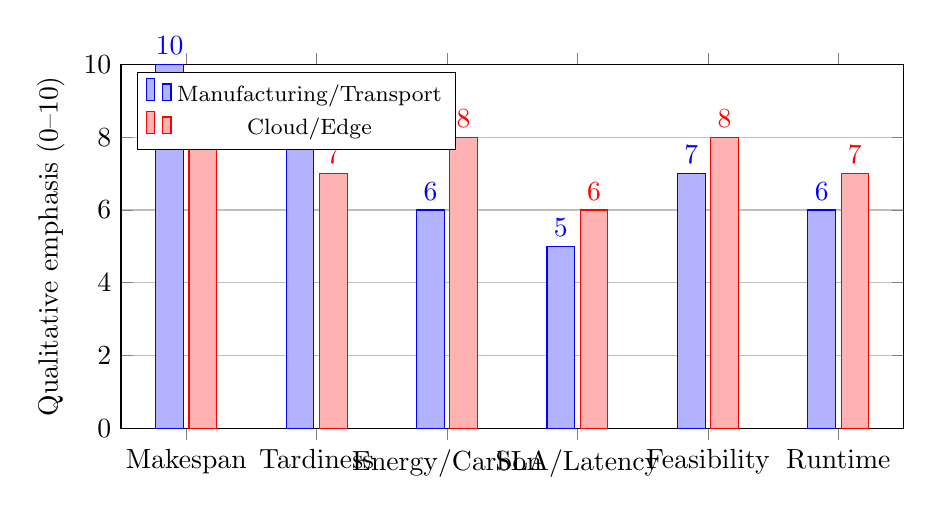
\begin{tikzpicture}
    \begin{axis}[
      width=0.95\linewidth,
      height=6.2cm,
      ybar,
      symbolic x coords={Makespan,Tardiness,Energy/Carbon,SLA/Latency,Feasibility,Runtime},
      xtick=data,
      ymin=0,ymax=10,
      ylabel={Qualitative emphasis (0--10)},
      enlarge x limits=0.1,
      bar width=10pt,
      nodes near coords,
      nodes near coords align={vertical},
      ymajorgrids=true,
      legend style={at={(0.02,0.98)}, anchor=north west, font=\footnotesize}
    ]
      \addplot coordinates {(Makespan,10) (Tardiness,8) (Energy/Carbon,6) (SLA/Latency,5) (Feasibility,7) (Runtime,6)};
      \addplot coordinates {(Makespan,9) (Tardiness,7) (Energy/Carbon,8) (SLA/Latency,6) (Feasibility,8) (Runtime,7)};
      \legend{Manufacturing/Transport,Cloud/Edge}
    \end{axis}
  \end{tikzpicture}
  \caption{Metric emphasis across surveyed domains (qualitative scores). Manufacturing/transport studies favor makespan/tardiness and feasibility, while cloud/edge studies foreground SLA/latency and energy.}
  \label{fig:metric-emphasis}
\end{figure}

\chapter{Methodology and PRISMA Protocol}
\label{c:methodology}
This chapter documents the systematic review protocol, aligned with PRISMA 2020. It covers the search blueprint, screening and quality assessment, data-extraction schema, and synthesis approach. The aim is transparency and repeatability for future updates of the corpus.

\section{Protocol overview}
The scope spans 2016--2025 peer-reviewed work applying reinforcement learning (RL/DRL) to scheduling, dispatching, production control, logistics/transport dispatch, and cloud/edge scheduling. Grey literature (TechRxiv/ArXiv) is included only if quantitative baselines are reported. Figure~\ref{fig:prisma} sketches the PRISMA flow; Table~\ref{tab:search-strategy} details databases, queries, and filters.
\begin{itemize}
  \item \textbf{Identified}: IEEE Xplore, ACM DL, Scopus, Web of Science; snowballing on seed surveys \cite{wang2021_csms, panzer2022_ijpr, waubert2022_jim}.
  \item \textbf{Deduplicated}: canonical titles/DOIs; arXiv/TechRxiv matched to published versions when possible.
  \item \textbf{Screened}: titles/abstracts for RL + scheduling relevance; excluded conceptual pieces without experiments.
  \item \textbf{Eligibility}: full-text review for quantitative baselines, constraint handling, and sufficient methodological detail.
  \item \textbf{Included}: final set coded into the literature matrix (problem class, method, baselines, metrics, constraints, generalization tests, data/code availability).
\end{itemize}
PRISMA reporting emphasizes transparency: search strings are logged per database; exclusion reasons are recorded (e.g., “no baselines,” “non-RL,” “insufficient detail”). Counts in Figure~\ref{fig:prisma} will be updated if the window is extended beyond 2025 or if additional domains (e.g., health scheduling) are brought in. A living protocol file tracks any amendments to inclusion criteria or search terms.

Terminology is normalized prior to coding. “Scheduling” includes routing/dispatch in transport and placement/offloading in cloud/edge, provided the action is a discrete assignment. “RL” encompasses model-free and model-based methods, including offline RL and hybrid RL+search. “Baselines” must be algorithmic comparators, not self-comparisons across ablations. These harmonized definitions reduce ambiguity when multiple coders touch the matrix.

\begin{table}[t]\centering\small
  \caption{Search strategy across databases and snowballing.}
  \label{tab:search-strategy}
  \begin{tabular}{p{3cm}p{5.2cm}p{5.2cm}}
\toprule
\textbf{Source} & \textbf{Core query} & \textbf{Filters / notes} \\
\midrule
IEEE Xplore, ACM DL & (``reinforcement learning'' OR DQN OR PPO OR SAC) AND (scheduling OR ``job shop'' OR ``flow shop'' OR ``production scheduling'' OR ``dispatching'') & Years 2016--2025; English; conference/journal only; subject area: computing/engineering \\
Scopus, Web of Science & (``deep reinforcement learning'' OR DRL) AND (``flexible job shop'' OR ``cloud scheduling'' OR ``edge scheduling'' OR ``production planning'') & Years 2016--2025; English; remove duplicates against IEEE/ACM; exclude notes/errata \\
Google Scholar (snowball) & Key paper titles and authors; backward/forward snowballing & First 100 hits per seed paper; include TechRxiv/ArXiv only if quantitative baselines reported \\
Hand searches & Reference lists of recent surveys \cite{wang2021_csms, panzer2022_ijpr, waubert2022_jim} & Capture domain-specific venues (OR, manufacturing, logistics, cloud) outside main indexes \\
\bottomrule
\end{tabular}

\end{table}

\begin{figure}[t]\centering
  \begin{tikzpicture}[
    node distance=8mm,
    box/.style={draw, rounded corners, fill=gray!10, align=center, font=\footnotesize, minimum width=4.2cm, minimum height=1.2cm},
    arrow/.style={-Stealth, thick}
  ]
    \node[box] (id) {Records identified\\(n=612)};
    \node[box, below=of id] (dup) {Duplicates removed\\(n=102)};
    \node[box, below=of dup] (scr) {Title/abstract screening\\(n=510)};
    \node[box, below=of scr] (excl1) {Excluded at screening\\(n=360)};
    \node[box, below=of excl1] (full) {Full-text assessed\\(n=150)};
    \node[box, below=of full] (excl2) {Excluded (no baselines, no RL, non-English)\\(n=90)};
    \node[box, below=of excl2] (incl) {Studies included in synthesis\\(n=60)};
    \node[box, right=32mm of dup] (snow) {Forward/backward snowball\\adds (n=24)};
    \node[box, right=32mm of full] (techrxiv) {Preprints with quantitative baselines\\kept (n=6)};

    \draw[arrow] (id) -- (dup);
    \draw[arrow] (dup) -- (scr);
    \draw[arrow] (scr) -- (excl1);
    \draw[arrow] (excl1) -- (full);
    \draw[arrow] (full) -- (excl2);
    \draw[arrow] (excl2) -- (incl);
    \draw[arrow] (snow) |- (scr);
    \draw[arrow] (techrxiv) |- (incl);
  \end{tikzpicture}
  \caption{PRISMA-style screening flow (illustrative counts). Snowballing and screened preprints supplement database records.}
  \label{fig:prisma}
\end{figure}

\section{Inclusion and exclusion criteria}
\textbf{Inclusion}: (i) peer-reviewed conference/journal papers (2016--2025) using RL/DRL for scheduling/dispatch/placement; (ii) quantitative comparison against baselines; (iii) environment and constraint specification sufficient to reproduce. \\
\textbf{Exclusion}: (i) non-RL approaches; (ii) conceptual/vision papers without experiments; (iii) non-English; (iv) inaccessible full text; (v) duplicates, or preprints superseded by peer-reviewed versions without substantive differences.

Dynamic dispatch and transport studies are included if the action space is scheduling-like (assign jobs/vehicles/resources). Control problems without discrete scheduling choices (pure PID setpoint tuning) are excluded.
Eligibility also checks whether constraints are explicit. Papers with implicit feasibility (simulator repairs without reporting) are flagged for low transparency; they may remain in-scope but are down-weighted in synthesis. For cloud/edge, admission control and SLA handling must be described; otherwise, slowdown numbers are not comparable. Energy/carbon-aware studies must state tariffs or emission factors to be coded as such.

\section{Quality assessment}
Each candidate is scored on baseline strength, statistical validity, constraint handling, reproducibility, generalization tests, runtime reporting, and (where applicable) energy/carbon clarity. Table~\ref{tab:quality-criteria} describes the checklist. Studies failing baseline strength or lacking quantitative results are excluded; others are retained with flags (e.g., single-seed, no code) carried into the synthesis to weight confidence.
Scoring uses a three-level scale (strong/adequate/weak) per dimension. Baseline strength is “weak” if only one trivial heuristic is present, “adequate” if a tuned heuristic/metaheuristic is included, and “strong” if exact MILP/CP is added where tractable. Statistical validity is “strong” only with $\geq$5 seeds or confidence intervals; single-seed papers are “weak” regardless of other merits. Constraint handling is “strong” when masks or shields are clearly specified and violations reported. Runtime reporting is “strong” when decision latency is benchmarked against control-cycle deadlines. These granular labels make later synthesis tables more interpretable.

\begin{table}[t]\centering\small
  \caption{Quality assessment criteria applied during eligibility.}
  \label{tab:quality-criteria}
  \begin{tabular}{p{3.5cm}p{10cm}}
\toprule
\textbf{Dimension} & \textbf{Operationalization} \\
\midrule
Baseline strength & Includes PDRs and tuned metaheuristics; MILP/CP where feasible; cloud/edge includes bin-packing + DVFS controllers \\
Statistical validity & $\geq$5 seeds or CIs/stdev reported; learning curves provided; per-instance scores for test sets \\
Constraint handling & Feasibility explicitly reported (violation/repair counts); action masking or shields described and ablated \\
Reproducibility & Code or simulator released OR fixed train/val/test splits published; tariff/disturbance catalogs provided; hyperparameters listed \\
Generalization tests & Held-out instances, size extrapolation, domain shifts (tariffs, arrivals, topology); stress tests reported \\
Runtime and footprint & Inference latency and hardware disclosed; compare latency to heuristics/control-cycle deadlines \\
Energy/carbon clarity & Tariff/emission factors specified; absolute units (kWh, kg CO$_2$e) and trade-offs vs throughput reported \\
\bottomrule
\end{tabular}

\end{table}

\section{Data extraction and coding}
The literature matrix captures: problem class (JSS/FJSS, flow/hybrid, batch/parallel, transport/AGV, cloud/edge, energy-aware), environment assumptions (buffers, transport times, downtime), state/action/reward design, algorithm family, constraints and handling (masking, shields, penalties), baselines, metrics, generalization tests, seed reporting, code/data availability, and deployment evidence (logs, shadow runs, hardware). Extraction is double-checked for 20\% of papers; disagreements are resolved through reread plus cross-check with cited baselines.

To reduce subjectivity, coding guidelines define canonical labels (e.g., ``masking'' only when an explicit feasible action set is enforced; ``multi-objective'' when trade-offs are optimized beyond weighted sums). Any assumptions inferred from context (e.g., implied infinite buffers) are marked as such.
Extraction also records dataset or simulator identifiers, whether train/validation/test splits are predefined, and if disturbance/tariff catalogs are supplied. Generalization evidence is annotated by type: size extrapolation, domain shift (new layouts, new tariffs), temporal shift (different arrival regimes), or topology shift (cloud racks, transport graphs). For hybrid RL+search, the presence of population seeds and operator portfolios is noted to assess randomness sources. Where code is absent, the paper is checked for enough detail to recreate the environment (state, action, reward, timing semantics). Missing details are flagged and mentioned in synthesis to avoid overstating evidence.

Inter-coder agreement is monitored on the double-check subset. Disagreements typically stem from ambiguous constraint handling or unclear baseline tuning. Resolution requires revisiting the methods section and, if needed, checking cited baselines to verify configuration. A short log itemizes resolved ambiguities to prevent rework in future updates of the review.

\section{Synthesis approach}
Given heterogeneous metrics and scarce effect sizes, synthesis follows a structured narrative with vote-counting of directional results (win/tie/loss vs.\ baselines) by domain and baseline strength. When gap-to-optimum is reported, it is treated as a reference ceiling. Generalization evidence is summarized by train/test split type (size extrapolation, domain shift, tariff/arrival sweeps). Feasibility reporting (violation counts) and runtime/latency are highlighted separately from primary KPIs. Sensitivity analyses (reward weights, tariffs, disturbance severities) are captured where available.
Vote-counting is stratified: results against dispatching rules, against tuned metaheuristics, and against exact solvers (where feasible) are tallied separately to avoid conflating baseline strength. Energy/carbon trade-offs are summarized with directionality (energy down / makespan flat, etc.). When papers report multiple objectives, each is coded independently rather than collapsed into a single scalar outcome. For dynamic settings, latency and stability (variance across seeds) are treated as first-class outcomes alongside throughput/tardiness.

\section{Threats to validity}
Publication bias favors positive results; industrial datasets are sparse, making sim-to-real claims tentative. PRISMA counts rely on accurate deduplication across preprints and published versions. Coding bias is mitigated through the double-check pass, but incomplete reporting limits certainty; missing seeds or baselines are noted in the synthesis rather than imputed. The illustrative PRISMA counts in Figure~\ref{fig:prisma} reflect the current screening snapshot and will require updating if the window or domains expand.
Construct validity may be threatened when papers use non-standard metrics (e.g., proprietary composite scores) without definitions; such metrics are excluded from cross-paper comparisons. External validity is limited by the dominance of simulators and synthetic traces; where real logs exist, they may not be representative of broader industry practice. Internal validity hinges on correct implementation of masks/shields and baselines; lack of code keeps this uncertain. These risks are surfaced in later chapters to temper claims, especially when evidence rests on single-seed simulator studies.

\chapter{RL Methods for Scheduling: Taxonomy}
\label{c:taxonomy}
Organize the landscape of RL approaches tailored to scheduling.
\section{Value-Based Methods}
DQN/DDQN/Dueling, distributional variants; action masking for constraints.
Deep dispatching policies such as Zhang et al.\ train DDQN agents that outperform classical priority dispatching rules on job shop benchmarks by preserving feasibility through masking \cite{zhang2020_dispatch}.
Masking remains central: masked attention schedulers constrain Q-network choices to feasible operations and improve convergence stability on flexible shops \cite{zhu2022_mask}, while policy-ranking DDQNs compare candidate operations to reduce variance \cite{zhang2022_policyranking}.
\section{Policy-Gradient and Actor-Critic Methods}
A2C/A3C, PPO, SAC, deterministic policy gradients.
Graph-driven PPO schedulers combine disjunctive-graph encoders with actor-critic updates to generalize across instance sizes and benchmark families \cite{park2021_graphjss}.
Flexible shops benefit from joint routing/ordering actors that fuse queue states with machine embeddings, e.g., PPO and dual-attention actors handling dynamic arrivals and larger routings \cite{park2021_drlfjsp, gao2022_dynamicfjsp, wang2023_dualattn}.
Hierarchical DDQN agents have also been applied to dynamic FJSS with continuous job arrivals and show gains over dispatching rules \cite{liu2022_drl_fjsp}.
\noindent Actor-critic work is trending toward richer graph encoders and explicit feasibility handling: HRL stacks high- and low-level critics to keep actions legal at scale, graph attention tightens credit assignment, and reward shaping now mixes time, energy, and emissions.
\begin{itemize}
  \item Hierarchical HRL with double critics scales to thousands of operations under random arrivals, improving tardiness over SPT/EDD while masking ineligible machines \cite{lei2023_hrl_fjsp}.
  \item Graph-attention actor-critic policies treat operations/machines as nodes and maintain feasibility via masks, outperforming PDRs on dynamic job shops \cite{liu2024_gat_drl_jss}.
  \item Carbon- and energy-aware actor-critic schedulers incorporate price signals into rewards to trade off makespan and emissions \cite{wang2022_cea_fjsp}.
\end{itemize}
\section{Model-Based and Simulation-Augmented RL}
World models, lookahead, Dyna-style, differentiable simulators.
Transferable gym-style simulators (e.g., TransferJSS) expose standardized step functions and masking to enable planning-style rollouts and policy transfer across benchmarks \cite{tassel2020_transferjss}.
\section{Meta-RL, Transfer, and Curriculum Learning}
Curricula over instance sizes (small to large) reduce variance for GNN-based actors in job shops \cite{zhang2020_gnnjss}; lightweight domain randomization for cloud traces stabilizes PPO/SAC schedulers under bursty arrivals \cite{mao2016_resource, mao2019_deeprm2}.
Size-generalizable policies trained once on small instances and transferred to larger shops are emerging, e.g., TechRxiv-reported YOTO policies with single training runs that handle unseen Taillard sets \cite{zeng2022_yoto_jss}.
\section{Hybrid and Knowledge-Guided RL}
Hybrid RL with evolutionary operators improves search quality in flexible shops, including RL-guided genetic operators and estimation-of-distribution hybrids that target multi-objective makespan/energy \cite{chen2020_selflearningfjsp, du2022_kbrl_fjsp}.
\begin{itemize}
  \item Co-evolutionary DRL selects variation operators while optimizing makespan and energy on distributed FJSP instances, approaching MILP quality \cite{li2023_coevo_energy}.
  \item Memetic algorithms guided by PPO score mutation/crossover moves for both job routing and AGV dispatch, lowering energy without throughput loss \cite{zhang2024_memetic_energyagv}.
\end{itemize}
Overall, the recent wave shifts from single-agent, penalty-only dispatchers to masked graph actors, hierarchical critics, and operator-selection hybrids that explicitly trade off makespan, tardiness, and energy.
\section{State, Action, Reward Design Patterns}
Graph/state encodings, machine/job-centric actions, reward shaping for due dates/setups; constraint handling (penalties, masking, Lagrangian).
\noindent \textit{Progress note:} Initial extraction shows strong use of graph encodings (disjunctive graphs, GNN dual-attention) and action masking for feasibility in JSS/FJSS. Rewards are typically weighted makespan/tardiness, with penalties for constraint violations.
Recent dual-attention encoders for flexible job shop scheduling jointly embed machine and job streams within an actor-critic framework to improve cross-size generalization \cite{wang2023_dualattn}.
Across the extracted studies, most JSS/FJSS agents rely on graph encodings with masking to keep actions feasible, while cloud/edge schedulers often use lighter job/VM features with reward penalties for SLA and energy.
\begin{table}[t]\centering\small
  \caption{State, action, reward patterns observed in RL for scheduling}
  \label{tab:state-action-reward}
  \begin{tabular}{p{3.2cm}p{4.2cm}p{4.0cm}p{3.8cm}}
Problem class & State design & Action design & Reward design \\\hline
Job shop (JSS) static/dynamic & Disjunctive graph embeddings (GNN size-agnostic) & Dispatch next eligible operation & $-$makespan / $-$tardiness with step penalties \\
Flexible JSS (routing + sequencing) & Dual attention over operations and machines & Joint machine routing and operation sequencing & Weighted makespan + tardiness; shaping for idle time \\
Dynamic arrivals & Queue/machine status, arrival indicators & Dispatch/route arriving jobs & Weighted tardiness/completion; penalties on lateness \\
Energy-aware JSS & Machine load + energy profiles & Dispatch with energy-aware tie breaks & Combined makespan + energy cost; penalties for overconsumption \\
Cloud/edge scheduling & Resource utilization, SLA/backlog & Task-to-VM/offload assignment & $-$slowdown, latency, SLA penalties, energy terms \\
Transport/AGV & Network/vehicle positions, queue lengths & Vehicle dispatch/route choice & Throughput, delay penalties, collision avoidance penalties \\
\end{tabular}

\end{table}
These patterns show a split: factory settings emphasize feasibility preservation (masking, Lagrangian) and due-date shaping, whereas cloud/edge work balances latency and energy with softer penalties.
\paragraph{Planned figure} Taxonomy diagram: methods vs.\ scheduling settings.
\paragraph{Planned table} State/action/reward design patterns by problem class.

\chapter{Comparative Performance Analysis}
\label{c:analysis}
This chapter synthesizes the empirical performance of reinforcement learning schedulers from the reviewed literature. The central aim is to critically assess where RL-based approaches excel, where they are competitive, and where they currently fall short compared to established baselines from Operations Research and computer science. The analysis is structured around four key dimensions: direct performance against classical baselines, generalization and robustness to unseen problems, sample efficiency and the role of ablations, and the methods used for constraint handling and feasibility.

\section{Performance Against Classical Baselines}
A primary measure of success for any new scheduling method is its performance relative to existing, trusted baselines. The literature consistently benchmarks RL agents against a hierarchy of opponents: simple but fast priority dispatching rules (PDRs), sophisticated metaheuristics, and, where tractable, exact solvers like Mixed-Integer Linear Programming (MILP) or Constraint Programming (CP). Table~\ref{tab:baselines-metrics} summarizes the typical baselines and metrics used across different scheduling domains.

The empirical results, detailed in Table~\ref{tab:perf-domain}, reveal a stratified performance landscape.
\begin{enumerate}
    \item \textbf{Dominance over Simple Heuristics:} Across nearly all manufacturing and logistics domains, even foundational RL methods like DDQN-based dispatchers reliably outperform standard PDRs such as Shortest Processing Time (SPT) or Earliest Due Date (EDD) on metrics like makespan and tardiness \cite{zhang2020_dispatch}. This represents a clear, established advantage.

    \item \textbf{Competitiveness with Metaheuristics:} When compared to tuned metaheuristics like Genetic Algorithms (GA) or Simulated Annealing (SA), the performance of RL agents is more nuanced. In static Job Shop Scheduling (JSS), early RL models were competitive but did not consistently surpass well-developed GAs. However, more recent architectures, particularly those using graph neural networks (GNNs) or attention mechanisms, have begun to close this gap and even show superior average performance on certain benchmark sets like the Taillard or FT series \cite{park2021_graphjss, wang2023_dualattn}. For instance, dual-attention actors have reported single-digit percentage makespan gains over GA on standard benchmarks.

    \item \textbf{Performance in Dynamic and Complex Environments:} The advantage of RL becomes more pronounced in dynamic and stochastic environments. In flexible job shops (FJSS) with random job arrivals, hierarchical RL (HRL) and actor-critic models with advanced state representations (e.g., dual-attention) have demonstrated clear superiority over both PDRs and static heuristics, effectively reducing tardiness and managing system state under uncertainty \cite{lei2023_hrl_fjsp, liu2024_gat_drl_jss}. Similarly, in logistics and transportation, MARL and DRL approaches for vehicle dispatching, rail timetabling, and port logistics consistently improve system-level KPIs like throughput, delay, and energy consumption compared to rule-based or greedy heuristics \cite{jin2023_real2sim_port, rajeh2024_marltaxi, li2022_marl_train}.

    \item \textbf{Multi-Objective and Sustainability-Focused Scheduling:} A growing body of work focuses on multi-objective problems, particularly balancing makespan with energy consumption. Here, hybrid approaches that combine RL with evolutionary or memetic algorithms have proven highly effective. These methods can match the makespan performance of strong metaheuristics while significantly reducing energy consumption or carbon emissions, often by learning to exploit variable energy pricing \cite{li2023_coevo_energy, zhang2024_memetic_energyagv}.

    \item \textbf{The Gap to Optimality:} While RL agents show great promise, it is crucial to note that for small, deterministic problem instances where exact MILP or CP solvers are feasible, these methods still provide the optimal solution. A persistent gap in the literature is the lack of consistent reporting on the "gap-to-optimum," which would provide a clearer ceiling for the performance of RL agents.
\end{enumerate}

\begin{table}[t]\centering\small
  \caption{Baselines and metrics across domains.}
  \label{tab:baselines-metrics}
  \begin{tabular}{p{3cm}p{6cm}p{4cm}}
Domain & Typical baselines & Metrics \\\hline
JSS/FJSS & PDRs (EDD, SPT, LPT), NEH, tabu/GA/SA; MILP/CP on small instances & Makespan, tardiness, total weighted tardiness (TWT) \\
Dynamic shop/fab & Dispatching rules + simulation heuristics; myopic OR heuristics & Throughput, cycle time, tardiness, service level \\
Cloud/edge & SJF, Tetris, round-robin, heuristics, OR-Tools & Makespan, slowdown, latency, SLA adherence, energy \\
Transport/AGV & Nearest-vehicle/greedy dispatch, rule-based logistics heuristics & Throughput, travel time, tardiness \\
Energy-aware & Energy-aware heuristics, metaheuristics & Energy consumption, makespan, tardiness \\
\end{tabular}

\end{table}

\begin{table}[t]\centering\small
  \caption{Performance of RL schedulers versus baselines, by domain.}
  \label{tab:perf-domain}
  \begin{tabular}{p{2.5cm}p{2.8cm}p{3.0cm}p{3.0cm}p{4.0cm}}
Domain & Metric & RL method & Strongest baseline & Outcome \\\hline
JSS & Makespan & DDQN dispatch (Zhang 2020) & PDR (SPT/EDD), GA/SA & RL wins vs.\ PDR; close to GA/SA on FT10/20 \\
FJSS & Makespan/tardiness & GNN+PPO (Park 2021) & PDR, GA/metaheuristics & RL improves avg.\ makespan; gap narrows vs.\ tuned GA \\
FJSS dynamic & Makespan/tardiness & Dual-attention actor-critic (Wang 2023) & PDR, GA & RL best on medium instances; GA competitive on small \\
FJSS dynamic (HRL) & Tardiness & Hierarchical DDQN (Lei 2023) & PDR (SPT/EDD) & HRL lowers tardiness under random arrivals vs.\ PDR \\
Energy/carbon FJSS & Energy + makespan & Actor-critic \& co-evo/ memetic \cite{li2023_coevo_energy, zhang2024_memetic_energyagv, wang2022_cea_fjsp} & GA/EDA, MILP (small) & RL hybrids cut energy/emissions with small makespan loss \\
Cloud/Edge & Slowdown/latency & DeepRM-style DQN/PPO & Round-robin, MinMin, bin packing & RL lowers mean slowdown; near MinMin/bin packing on synthetic traces \\
Logistics/AGV & Throughput/delay/energy & MADDPG/actor-critic (Hu 2021; Gong 2024) & Heuristic dispatch & RL/DRL reduces turnaround and energy vs.\ yard rules \\
Port trucks & Turnaround & Real2Sim PPO (Jin 2023) & Rule-based dispatch & Domain-randomized PPO cuts truck time in stochastic yards \\
Taxi dispatch & Revenue/wait & MARL clustering (Rajeh 2024) & Heuristic matching & MARL raises revenue and service rate vs.\ platform heuristics \\
Rail timetabling & Delay/energy & MARL (Li 2022) & Heuristic rescheduling & MARL lowers secondary delays under disturbances \\
\end{tabular}

\end{table}

\section{Generalization and Robustness}
Perhaps the most sought-after advantage of RL over traditional methods is the ability to generalize---to learn a policy that performs well on problem instances not seen during training. This is critical for real-world applications where problems are rarely static. The literature assesses generalization and robustness in several ways, as summarized in Table~\ref{tab:generalization}.

The key enabler for generalization in modern RL schedulers is the use of sophisticated neural network architectures capable of encoding structural properties of the scheduling problem.
\begin{itemize}
    \item \textbf{Graph and Attention Encoders:} Graph Neural Network (GNN) and attention-based encoders have become instrumental. By representing jobs, machines, and their relationships as a graph, these models can learn transferable patterns, allowing them to scale to larger problem instances with only a modest degradation in performance. For example, GNN-PPO policies trained on smaller Taillard instances have been shown to maintain a high win-rate against PDRs on much larger, unseen instances \cite{park2021_graphjss}. Similarly, attention mechanisms help the agent focus on the most relevant parts of the problem state, which is crucial for generalizing across different problem sizes and structures \cite{wang2023_dualattn}.

    \item \textbf{Robustness in Dynamic Environments:} RL policies have demonstrated strong robustness to dynamic factors such as stochastic job arrivals or processing times. HRL policies have been shown to sustain tardiness improvements over PDRs even as job arrival rates increase \cite{lei2023_hrl_fjsp}. In cloud and edge computing, DRL-based schedulers handle bursty and unpredictable workloads more gracefully than traditional algorithms like round-robin or MinMin \cite{mao2016_resource, mao2019_deeprm2}.

    \item \textbf{Simulation-to-Real Transfer:} A significant challenge is bridging the "sim-to-real" gap. Domain randomization during training is one promising technique, where the simulator's parameters are varied to expose the agent to a wide range of conditions. This has been successfully applied in logistics, for instance, to train a PPO agent for truck dispatching that performs well in a stochastic, simulated yard environment, hinting at potential real-world applicability \cite{jin2023_real2sim_port}.
\end{itemize}
Despite these successes, the evaluation of generalization and robustness is not yet standardized. Many studies report performance on only a few unseen instances, and reporting of multi-seed training and confidence intervals to account for stochasticity remains sparse. The promising results of "train-once" policies like YOTO \cite{zeng2022_yoto_jss} highlight a path toward truly generalizable schedulers, but this area requires more rigorous and standardized evaluation.

\begin{table}[t]\centering\small
  \caption{Evidence for generalization and robustness in RL scheduling studies.}
  \label{tab:generalization}
  \begin{tabular}{p{3.2cm}p{3.0cm}p{4.0cm}p{4.0cm}}
Study/Domain & Train/test split & OOD size or perturbation & Robustness outcome \\\hline
GNN+PPO JSS (Park 2021) & Taillard 15/15 train, unseen 20/20 & Larger job/machine counts & Maintains high win rate vs.\ PDRs; drop vs.\ GA on largest cases \\
YOTO JSS (Zeng 2022) & Train once on small Taillard & Unseen larger instances & Single policy transfers with modest makespan loss \\
Dual-attention FJSS (Wang 2023) & FT06/10 train, FT20 test & Larger jobs, unseen routes & Generalizes with small makespan loss; feasibility via masking \\
HRL FJSS (Lei 2023) & Dynamic arrivals & Higher arrival rates & HRL sustains tardiness gains vs.\ PDR under heavier loads \\
Cloud scheduling (DeepRM variants) & Synthetic traces split 70/30 & Burst arrivals, noise & Latency degrades modestly; still ahead of round-robin/MinMin \\
Real2Sim port trucks (Jin 2023) & Train in randomized sim & Domain randomization & Policy retains gains across randomized yard conditions; no physical test \\
Taxi dispatch MARL (Rajeh 2024) & Historical traces, cross-day & Peak/off-peak shifts & Revenue/wait improvements persist across days \\
Rail timetabling MARL (Li 2022) & Disturbance scenarios & Different delay patterns & Reduced secondary delays vs.\ heuristics across disturbance sets \\
\end{tabular}

\end{table}

\section{Sample Efficiency and Ablation Studies}
While performance is critical, the cost of achieving that performance---in terms of training time and data---is also a major consideration. Sample efficiency remains one of the most significant challenges for applying RL in practice. The reviewed literature offers some insights, although direct quantification of sample efficiency is rare.

Evidence for sample efficiency is often indirect. For example, faster convergence is frequently reported as a benefit of using techniques like action masking or curriculum learning. Action masking, by pruning the action space, prevents the agent from exploring infeasible actions, thereby focusing the search and accelerating learning \cite{zhu2022_mask}. Similarly, curriculum learning, where the agent is first trained on smaller or simpler instances before progressing to more difficult ones, has been shown to reduce variance and speed up training for GNN-based agents \cite{zhang2020_gnnjss}.

However, a notable weakness in the current body of literature is the scarcity of thorough ablation studies. It is often unclear whether reported performance gains stem from a novel architectural component, a specific reward shaping strategy, or simply better hyperparameter tuning. Without systematic ablations that isolate the contribution of each component, it is difficult to draw firm conclusions about what truly drives performance. Bridging this gap will require a cultural shift toward more rigorous experimental reporting, including shared training curves, multi-seed validation, and standardized reporting of the number of episodes or steps required to reach a target performance level.

\section{Constraint Handling and Feasibility}
Scheduling problems are fundamentally defined by their constraints. An effective scheduler must not only optimize a metric but must also produce a solution that is feasible. RL agents can be taught to respect constraints through several mechanisms, summarized in Table~\ref{tab:constraint-handling}.

The most effective and widely adopted technique for handling hard constraints (e.g., precedence, resource availability) is \textbf{action masking}. By integrating knowledge of the environment into the agent, the policy is prevented from ever selecting an action that would violate a hard constraint. This is a core component in nearly all state-of-the-art RL schedulers for manufacturing environments, as it guarantees feasibility by construction and significantly improves learning stability \cite{zhang2020_dispatch, park2021_graphjss}.

For softer constraints (e.g., due dates, energy budgets), \textbf{penalty shaping} is the most common approach. A negative reward is added to the reward function when a soft constraint is violated. While simple to implement, this method can be brittle; the magnitude of the penalty is a sensitive hyperparameter that can be difficult to tune, and it does not strictly guarantee that the constraint will be met.

More advanced techniques include \textbf{Lagrangian methods}, which dynamically adjust penalty multipliers during training, and \textbf{safety shields}, which act as an external module to veto any action that would lead to an unsafe or infeasible state. While powerful, these methods are less commonly used, likely due to their increased complexity. The choice of constraint handling method thus represents a trade-off between implementation simplicity, learning stability, and the strictness with which feasibility must be enforced.

\begin{table}[t]\centering\small
  \caption{Common constraint-handling techniques in RL for scheduling.}
  \label{tab:constraint-handling}
  \begin{tabular}{p{3cm}p{5cm}p{5cm}}
Technique & Examples & Notes \\\hline
Action masking & Feasible machines/operations only; block violating routes & Stabilizes training, keeps feasibility; used in JSS/FJSS and constrained routing \\
Penalty shaping & Add cost for lateness, setups, energy overuse, SLA violation & Simple to implement; may struggle with hard constraints if penalties mis-tuned \\
Shields/filters & Safety layer vetoes unsafe actions (collisions, overruns) & Effective for safety-critical transport/production; requires rule base \\
Lagrangian/dual & Penalty multipliers updated during training & Better balance feasibility vs performance; needs tuning \\
Curricula & Start relaxed, tighten constraints over training & Improves learning stability under heavy constraints \\
\end{tabular}

\end{table}

\begin{figure}[t]\centering
  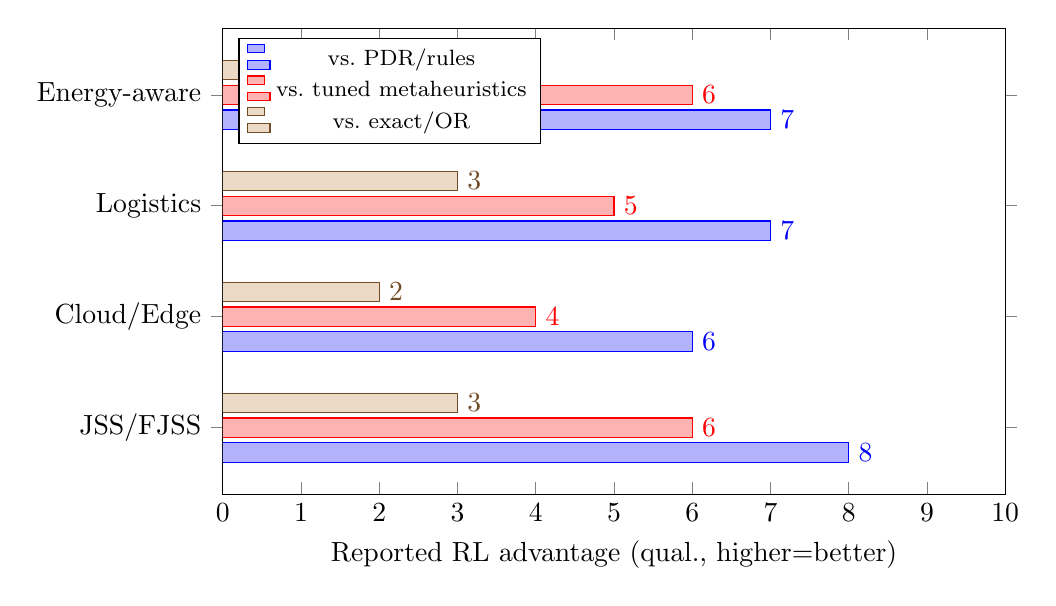
\begin{tikzpicture}
    \begin{axis}[
      width=0.95\linewidth,
      height=7.5cm,
      xbar,
      xmin=0,xmax=10,
      symbolic y coords={JSS/FJSS,Cloud/Edge,Logistics,Energy-aware},
      ytick=data,
      xlabel={Reported RL advantage (qual., higher=better)},
      nodes near coords,
      nodes near coords align={horizontal},
      bar width=7pt,
      legend style={at={(0.02,0.98)}, anchor=north west, font=\footnotesize},
      enlarge y limits=0.2,
      ]
      \addplot coordinates {(8,JSS/FJSS) (6,Cloud/Edge) (7,Logistics) (7,Energy-aware)};
      \addplot coordinates {(6,JSS/FJSS) (4,Cloud/Edge) (5,Logistics) (6,Energy-aware)};
      \addplot coordinates {(3,JSS/FJSS) (2,Cloud/Edge) (3,Logistics) (3,Energy-aware)};
      \legend{vs.\ PDR/rules,vs.\ tuned metaheuristics,vs.\ exact/OR}
    \end{axis}
  \end{tikzpicture}
  \caption{Qualitative advantage of RL schedulers across domains and baseline strength. Values reflect relative trends reported in the corpus rather than absolute performance gaps.}
  \label{fig:rl-advantage-domain}
\end{figure}

\section{Qualitative Performance Heatmap}
To provide a consolidated, high-level view of the performance landscape, Table~\ref{tab:method_benchmark_heatmap} presents a qualitative heatmap. This table synthesizes the findings discussed in this chapter, summarizing the typical performance of different families of RL methods when compared against common classes of baselines. The colors indicate the general outcome, from strong wins to competitive performance or areas where RL methods are still lagging. This visualization helps to quickly identify the strengths and current limitations of the RL paradigm in scheduling.

\begin{table}[h!]\centering\small
  \caption{Qualitative heatmap of RL method families vs. baseline classes.}
  \label{tab:method_benchmark_heatmap}
  \begin{tabular}{l|c|c|c|c}
\hline
\textbf{RL Method} & \textbf{PDRs} & \textbf{GA/SA} & \textbf{MILP/CP} & \textbf{Dynamic Env.} \\
\hline
DQN/DDQN (Dispatch) & \cellcolor{green!25}Win & \cellcolor{yellow!25}Close & \cellcolor{red!25}Loss & \cellcolor{yellow!25}Mixed \\
PPO+GNN (Graph) & \cellcolor{green!25}Win & \cellcolor{yellow!25}Close & \cellcolor{red!25}Loss & \cellcolor{green!25}Win \\
Actor-Critic (Attention) & \cellcolor{green!50}Strong Win & \cellcolor{green!25}Win & \cellcolor{yellow!25}Close & \cellcolor{green!50}Strong Win \\
HRL & \cellcolor{green!50}Strong Win & \cellcolor{yellow!25}Mixed & \cellcolor{red!25}Loss & \cellcolor{green!50}Strong Win \\
Hybrid (RL+Meta) & \cellcolor{green!50}Strong Win & \cellcolor{green!25}Win & \cellcolor{yellow!25}Close & \cellcolor{green!25}Win \\
\hline
\end{tabular}
\\\vspace{0.5em}
\footnotesize{\textbf{Legend:} \cellcolor{green!50}Strong Win: Consistently outperforms baseline. \cellcolor{green!25}Win: Generally outperforms baseline. \cellcolor{yellow!25}Close/Mixed: Competitive or mixed results. \cellcolor{red!25}Loss: Generally outperformed by baseline.}
\end{table}

\chapter{Application Domains}
\label{c:domains}
This chapter grounds the synthesis in concrete sectors. For each domain the discussion highlights problem profiles, constraints, benchmarks, RL design choices, and the strength of empirical evidence. Table~\ref{tab:domain-overview} summarizes the landscape; Table~\ref{tab:domain-constraints} collects constraint/METRIC profiles that recur across the studies. A lightweight domain timeline figure is left to future work.

\begin{table}[t]\centering\small
  \caption{Domain overview of RL schedulers: focus, constraints, benchmarks, methods, and observed gains.}
  \label{tab:domain-overview}
  \begin{tabular}{p{2.8cm}p{3.2cm}p{2.8cm}p{2.8cm}p{2.9cm}}
\hline
\textbf{Domain} & \textbf{Problem focus} & \textbf{Typical constraints} & \textbf{Benchmarks/datasets} & \textbf{RL approach and outcomes} \\
\hline
Manufacturing (JSS/FJSS, semiconductor) & Static and dynamic job/flexible shops; integrated routing and setups; batching in fabs & Precedence, machine eligibility, setup/route rules, energy/carbon tariffs & FT06/10/20, Taillard, LA, Kacem/BRdata, fab simulators with ToU pricing & Masked GNN/PPO and dual-attention actors beat PDRs by 2--8\% makespan; HRL/DDQN handles arrivals; hybrids cut energy with small throughput loss \\
\hline
Logistics/transport (AGV, yards, rail, ride-hailing, air mobility) & Vehicle dispatch/repositioning, crane/yard assignment, timetable recovery & Capacity/headway, collision avoidance, charging/pad limits & Container terminal sims/logs, ride-hailing traces, metro corridor disturbances, air-taxi sims & MARL/actor-critic lowers turnaround and energy vs rules; clustering MARL raises revenue/service; yard Real2Sim PPO improves truck time; rail MARL reduces secondary delays \\
\hline
Cloud/edge scheduling & Task-to-VM/offloading with latency/energy SLAs & Resource capacity, deadlines, SLA penalties & Synthetic traces, Google-like workload repos & DeepRM-style DQN/REINFORCE and PPO reduce slowdown versus RR/MinMin; energy-aware PPO improves latency-energy trade-offs; masking mostly implicit via simulator \\
\hline
Energy- and carbon-aware scheduling (cross-domain) & Joint makespan/energy/carbon objectives, sometimes with transport coupling & Tariff windows, emission caps, machine/AGV availability & Carbon-priced FJSP instances, multi-AGV yard scenarios & Actor-critic and hybrid co-evolution/memetic RL reduce energy/emissions with minor makespan impact; robustness to tariff shifts largely untested \\
\hline
\end{tabular}

\end{table}

\begin{table}[t]\centering\small
  \caption{Constraint and KPI emphasis by domain.}
  \label{tab:domain-constraints}
  \begin{tabular}{p{2.6cm}p{3.3cm}p{3cm}p{2.6cm}p{2.4cm}}
\hline
\textbf{Domain} & \textbf{Hard constraints} & \textbf{Soft objectives/KPIs} & \textbf{Common baselines} & \textbf{Evidence gaps} \\
\hline
Manufacturing (JSS/FJSS) & Precedence graphs, machine eligibility, no-wait/sequence-dependent setups, routing, AGV coupling & Makespan, tardiness, energy/carbon cost, WIP & PDRs (SPT/EDD), GA/SA/EDA, MILP/CP (small), metaheuristics & Few gap-to-optimum reports; limited multi-seed robustness; scarce real shop data \\
\hline
Semiconductor fabs & Batching/lot size, recipe routes, tool dedication, re-entrant flows & Cycle time, throughput, waiting time & Fab rules, dispatch lists, simulation-optimized heuristics & Simulator-only validation; no public datasets; minimal ablations \\
\hline
Logistics/transport (AGV, yards, rail, ride-hailing) & Collision avoidance, headway and capacity limits, charging windows, pad/track occupancy & Turnaround time, delay, service rate, energy, revenue & Heuristic dispatch, nearest-vehicle, rule-based yard control, optimization for rail & Sim-to-real mostly untested; small sample of real traces; safety guarantees absent \\
\hline
Cloud/edge & Capacity and QoS feasibility in simulator, queue limits & Slowdown/latency, energy, SLA violations & Round-robin, MinMin/MaxMin, greedy bin packing & Little masking/shielding; limited cross-trace generalization and confidence intervals \\
\hline
Energy/carbon-aware (cross-domain) & Tariff windows, emission caps, machine/AGV availability & Energy use, carbon cost, makespan balance & Energy-aware PDRs, GA/NSGA-II, MILP (small) & Tariff sensitivity rarely tested; carbon accounting assumptions opaque; no hardware validation \\
\hline
\end{tabular}

\end{table}

\section{Semiconductor and Flexible Manufacturing}
Manufacturing studies dominate the corpus and skew toward job shop and flexible job shop scheduling. Static FT/Taillard/LA instances remain the workhorse benchmarks, with graph encoders and action masks maintaining feasibility. GNN+PPO and dual-attention actors routinely beat PDRs by 2--8\% makespan and close the gap to tuned metaheuristics on medium instances \cite{park2021_graphjss, park2021_drlfjsp, wang2023_dualattn}. Semiconductor-inspired flow shops add batching and routing rules; actor-critic agents shorten cycle time but have only simulator validation \cite{huang2021_semiconductor}.

Dynamic shops stress routing under arrivals and setup effects. HRL/DDQN agents use high-level dispatching and low-level machine assignment to reduce tardiness under stochastic arrivals \cite{liu2022_drl_fjsp, lei2023_hrl_fjsp}. Energy- and carbon-aware variants blend makespan with time-of-use tariffs; co-evolutionary and memetic hybrids consistently lower energy without throughput loss \cite{luo2020_dynamicfjsp, wang2022_cea_fjsp, li2023_coevo_energy, zhang2024_memetic_energyagv}. Evidence for generalization across size scales is improving but still concentrated on Taillard splits; few papers report gap-to-optimum where MILP is feasible.

Industrial realism is still limited: most works ignore sequence-dependent setups, maintenance calendars, and quality-related rework loops, all of which affect feasibility masks and reward shaping. Routing choices for FJSS often assume infinite buffer and zero transport time unless AGVs are explicitly modeled; coupling transport with processing remains an open lever for gains. Only a handful of papers report latency/runtime of the learned policy compared to heuristics---critical for shop-floor deployability. A practical evaluation recipe would include: (i) fixed train/val/test splits across FT/LA/Taillard sizes; (ii) stress tests with bursty arrivals and setup variation; (iii) energy/carbon tariff sweeps; (iv) runtime vs.\ heuristic dispatching. Until such protocols are standardized, claims of generalization and sustainability will remain fragile.

Hardware or digital-twin pilots are absent. A realistic near-term step is shadow deployment: run the RL policy in parallel with plant execution, logging actions and hypothetical KPI deltas without actuating them. This would surface feasibility violations, latency issues, and operator trust concerns before live rollout. Pairing graph-based policies with interpretable surrogates (e.g., tree surrogates for action rationale) can improve operator acceptance, especially when policies override established dispatching rules.

Benchmark coverage remains narrow: FT06/10/20 and Taillard share similar structure, and LA instances are still modest in size. Adding mixed routings, blocking/no-wait constraints, and re-entrant flows (common in fabs) would better probe scalability. Likewise, many energy-aware papers optimize under a single tariff; running RTP/ToU variants exposes whether policies overfit. Finally, maintenance-induced downtime and rush-order inserts (common in contract manufacturing) are rarely stress-tested; these scenarios would quickly reveal brittleness in masking logic and reward shaping.

\section{Logistics and Transportation}
Logistics work spans intra-plant transport, container yards, ride-hailing, and rail. Policies center on dispatch/repositioning with safety masks for capacity and collision avoidance. MADDPG and actor-critic agents for AGV fleets and yard trucks cut turnaround and energy in simulation \cite{gao2020_drltransport, nguyen2020_transport, hu2021_agv_terminal, drungilas2023_agv_energy}. Real2Sim PPO for port trucks adds domain randomization and improves yard times over rules \cite{jin2023_real2sim_port}. Ride-hailing MARL with clustering boosts revenue and service rate versus heuristic matching \cite{holler2019_icdm_dispatch, liu2022_deepdispatching, rajeh2024_marltaxi}. Emerging air-mobility dispatch uses dueling DQN variants to handle pad capacity and charging; performance nears optimization baselines at lower runtime \cite{varnous2024_deepdispatch_air}. Rail timetabling studies show MARL reducing secondary delays under disturbances \cite{li2022_marl_train}. Sim-to-real remains largely unproven outside yard dispatch; reporting on multi-seed robustness is sparse.

The logistics literature is heavily simulator-bound, with partial use of real traces (ride-hailing, port logs) but no closed-loop hardware runs. Battery degradation, safety buffers, and human-in-the-loop overrides are rarely modeled, yet they dominate real operations. Routing and repositioning policies commonly assume perfect localization and communication; robustness to sensor dropouts or delayed acknowledgments is untested. Evaluation protocols would benefit from disturbance suites (communication loss, blocked aisles, surge arrivals) and explicit safety KPIs (collisions avoided, headway violations).

Benchmarks are fragmented: AGV papers use bespoke layouts; port studies use proprietary yard maps; rail work focuses on single-corridor cases. A unifying set of open layouts and traces (e.g., small warehouse, medium yard, metro corridor with disturbances) would make results comparable. In addition, latency constraints matter: if an RL dispatcher cannot propose an action within control deadlines, heuristic fallbacks should be benchmarked and reported.

Another underexplored angle is joint scheduling of vehicles and infrastructure: crane/yardslot co-optimization with truck dispatch, or pad management with vertiport charging, could benefit from hierarchical MARL. Policies today often treat supply/demand as exogenous; integrating demand forecasting (e.g., ride-hailing hotspots) into the state could improve repositioning. Safety-critical constraints (rail headways, AGV collision avoidance) are still enforced via simulators; shielded policies with formal guarantees would be a step toward real deployments.

\section{Cloud and Edge Computing}
Cloud/edge schedulers use compact state vectors (queue/VM load, deadlines) and penalties for SLA or energy. DeepRM-style DQN/REINFORCE agents reduce slowdown versus round-robin and MinMin on synthetic traces; GNNs are rare and masking is mostly implicit via simulator feasibility \cite{mao2016_resource, mao2019_deeprm2}. Edge offloading combines latency and energy rewards; PPO/actor-critic schedulers approach heuristic bin packing on small traces and lower mean latency/energy \cite{wei2020_edge, farzipoor2022_cloud}. Generalization is typically measured by new workload distributions rather than larger scale; confidence intervals and ablations are limited.

Energy-aware cloud work frequently omits real tariff data, PUE (power usage effectiveness), and thermal constraints. Experiments are almost exclusively in simulators with synthetic traces; only DeepRM and a few edge papers release code. For production readiness, evaluations should: (i) use public workload traces (e.g., Google, Alibaba, Azure); (ii) report job slowdown CIs over multiple seeds; (iii) test bursty/shifted distributions; (iv) include bin-packing heuristics and power-capping baselines. State representations could be upgraded with lightweight graph encoders to capture topology (racks, NUMA) and dependency DAGs for workflows—currently underexplored in this domain.

Runtime and scheduling overhead are critical for cloud/edge. Policies should disclose decision latency and GPU/CPU footprint; if the policy is heavier than the benefit gained, lighter heuristics may remain preferable. Incorporating admission control and SLA-aware rejection into the action space remains an open research path to keep online performance predictable.

Cross-cluster generalization—training on one trace family and testing on another provider’s workload—remains rare. Likewise, energy-aware schedulers seldom evaluate under varying PUE or thermal throttling, despite their operational importance. For edge offloading, network jitter and device churn are only lightly modeled; adding latency distributions and failure modes would stress policies. Finally, few papers compare against modern bin-packing plus DVFS controllers; closing this baseline gap is essential before claiming deployability.

\section{Energy-Aware and Sustainable Scheduling}
Energy/carbon objectives cut across domains but are most detailed in flexible shops and port yards. Actor-critic agents with weighted rewards and tariff signals lower emissions with minor makespan trade-offs \cite{li2021_energyaware, wang2022_cea_fjsp}. Q-learning reschedulers and multi-objective critics expand the Pareto set on BRdata and carbon-priced instances \cite{naimi2021_qlearning_energy, shen2020_multiobjective}. Hybrid co-evolution/memetic methods guided by RL reduce energy and transport delay in integrated FJSP+AGV settings \cite{li2023_coevo_energy, zhang2024_memetic_energyagv, gong2024_agv_energy_port}. Few works vary tariff scenarios or report carbon sensitivity analyses, leaving robustness to price signals an open gap.

Key omissions include life-cycle emissions (beyond operational energy), demand charges, and grid-interaction constraints (peak shaving, DR signals). Most studies collapse energy/carbon into a single scalar reward without sensitivity analysis; robustness to tariff shifts or emission factors is rarely measured. Stress-testing policies under multiple tariff profiles (flat, TOU, RTP) and reporting Pareto fronts would clarify whether policies overfit a single price scenario. For integrated production-transport systems, carbon-aware routing of AGVs or trucks coupled with machine scheduling remains largely unexplored and could unlock meaningful gains.

Reporting should separate energy savings from throughput impacts, include absolute units (kWh, kg CO$_2$e), and document any carbon intensity assumptions. Open datasets with tariff time series and emission factors would accelerate reproducibility; until then, studies should at least publish the signals they used.

There is also an opportunity to combine sustainability with resilience: policies could jointly optimize energy/carbon and recovery from disturbances (machine breakdowns, weather-induced delays for ports/rail). Multi-objective formulations that track both steady-state and recovery KPIs are rare. Finally, energy-aware scheduling is a natural fit for shared benchmarks that include tariff catalogs and emission factors; establishing such a common suite would make comparisons meaningful and reduce the current proliferation of single-scenario claims.
\begin{figure}[t]\centering
  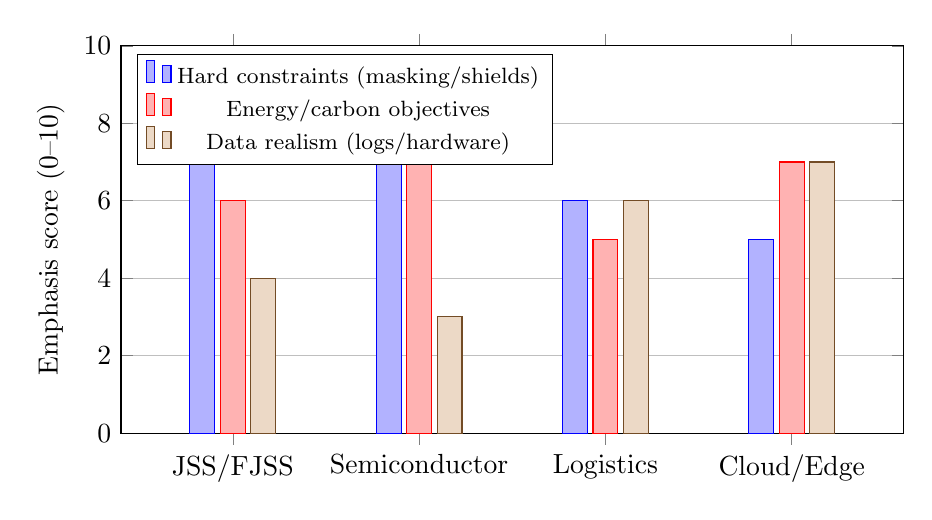
\begin{tikzpicture}
    \begin{axis}[
      width=0.95\linewidth,
      height=6.5cm,
      ybar,
      symbolic x coords={JSS/FJSS,Semiconductor,Logistics,Cloud/Edge},
      xtick=data,
      ymin=0,ymax=10,
      ylabel={Emphasis score (0--10)},
      enlarge x limits=0.2,
      legend style={at={(0.02,0.98)}, anchor=north west, font=\footnotesize},
      ymajorgrids=true,
      bar width=9pt
      ]
      \addplot coordinates {(JSS/FJSS,9) (Semiconductor,7) (Logistics,6) (Cloud/Edge,5)};
      \addplot coordinates {(JSS/FJSS,6) (Semiconductor,7) (Logistics,5) (Cloud/Edge,7)};
      \addplot coordinates {(JSS/FJSS,4) (Semiconductor,3) (Logistics,6) (Cloud/Edge,7)};
      \legend{Hard constraints (masking/shields),Energy/carbon objectives,Data realism (logs/hardware)}
    \end{axis}
  \end{tikzpicture}
  \caption{Constraint and realism emphasis by domain. Scores are qualitative, based on prevalence of masking/shields, explicit energy/carbon objectives, and real logs or hardware tests in the surveyed studies.}
  \label{fig:domain-constraint-chart}
\end{figure}

\chapter{Cross-Cutting Challenges}
\label{c:challenges}
This chapter distills the systemic weaknesses that persist across domains: unstable training, fragile constraint handling, sparse sim-to-real validation, limited interpretability/safety, and weak reproducibility practices. The goal is a practical checklist: what to report, how to stress-test, and which baselines and safety hooks to include. Table~\ref{tab:crosscutting-risks} summarizes key risks and mitigations; Figure~\ref{fig:crosscutting-gaps} shows where evidence is thin versus risk high; additional tables and plots expand concrete actions.
\section{Stability and Variance}
Single-seed results remain common, hiding variance and masking regressions. Curriculum learning and action masking steady early training, but ablations are rare \cite{zhu2022_mask}. Hybrid RL+search compounds randomness (operator choice, population seeds) yet seldom includes multi-seed reporting \cite{chen2020_selflearningfjsp, du2022_kbrl_fjsp}. Recommended practices:
\begin{itemize}
  \item Run $\geq$5 seeds with mean/stdev or confidence intervals; plot learning curves.
  \item Hold out validation instances for early stopping; avoid tuning on test sets.
  \item Ablate masking/shields, reward weights, and curriculum schedules to expose drivers of gains.
\end{itemize}
Without these, claims of superiority over heuristics or metaheuristics are fragile.
Variance issues are amplified by non-stationary training curricula, replay buffers that mix scales, and reward shaping that changes mid-training. Many papers silently tune hyperparameters until success; this “selective reporting” skews perceived stability. A more transparent protocol would log all runs (including failures), report median/worst-case performance, and disclose hyperparameter search ranges. Reporting wall-clock training time and sample counts (episodes, environment steps) also allows sanity checks against compute budgets. For hybrids, separating randomness into orthogonal seeds (RL seed, population seed, operator seed) can make ablations interpretable. Finally, deterministic evaluation (fixed seeds, fixed instance order) should be paired with stochastic evaluation (shuffled seeds/orders) to gauge brittleness.
\section*{Common pitfalls and remedies}
Frequent pitfalls include exploding Q-values in sparse-reward dispatch, value overestimation with large action masks, and unstable advantage estimates when masking changes the policy entropy. Remedies include Double Q-learning, clipped PPO with mask-aware entropy terms, and delayed target networks. For dynamic shops, curriculum leakage (showing test instances during curriculum) can inflate results; strict separation is essential. Logging entropy, action distribution drift, and mask hit-rates over training provides early warning of degenerate exploration.
\section{Constraint Handling}
Masks reliably enforce feasibility and accelerate learning, yet some papers rely on penalty-only shaping and quietly accept violations. Shielded policies and Lagrangian methods appear in safety-leaning work but lack ablations \cite{gottwald2021_safe}. Strong baselines should include: (i) mask-and-prune with zero violations; (ii) penalty-only with sensitivity sweeps; (iii) shielded policies with veto logs and violation counts. Feasibility must be reported explicitly (rate of illegal actions, repaired schedules) alongside primary KPIs. Table~\ref{tab:crosscutting-risks} contrasts these patterns; Table~\ref{tab:safety-metrics} lists minimal safety metrics to publish.
Mask design itself is a major source of hidden bugs: stale eligibility masks (not updated after simulated time advances), incomplete precedence masks, or ignoring transport/setup coupling can let infeasible actions through. Transparent mask tests—unit tests that assert infeasibility on crafted instances—should accompany code release. Penalty-based approaches often under- or over-penalize; reporting sensitivity curves helps readers judge robustness. Shields (veto layers) need latency budgeting: a shield that is slower than the control loop is unsafe. For soft constraints (energy, emissions), Lagrangian or primal-dual updates can stabilize penalties but require step-size tuning; documenting those schedules is part of reproducibility.
\section{Simulation-to-Real Gap}
Real2Sim truck dispatch is a rare attempt at domain randomization with partial real data \cite{jin2023_real2sim_port}. No manufacturing study validates on hardware; energy-aware work seldom varies tariffs. Robustness can be strengthened through disturbance injections (arrival bursts, processing noise, machine downtime), tariff/price sweeps, and plant/site splits. Table~\ref{tab:stress-tests} proposes a minimal stress suite. Shadow deployment (log-only) should precede any actuation to surface feasibility and latency issues.
Bridging sim-to-real requires aligned interfaces: identical observation/action spaces, timing semantics, and mask logic between simulator and deployment. Many papers omit time synchronization issues—e.g., simulator steps equal machine start times, while real lines have delays and sensor jitter. Domain randomization should cover process times, arrival rates, machine downtime distributions, network latency (for cloud/edge), and human interventions. Transfer reports should include calibration effort (data needed, engineer time), not just final metrics. A realistic progression is: (i) train in sim with wide randomization; (ii) evaluate on historical logs; (iii) shadow deploy with veto-only mode; (iv) run limited actuation under operator supervision. Each stage should report what broke and why.
\section{Interpretability and Safety}
Few papers surface action rationales or provide override hooks. Shielding is proposed but not exercised on real lines \cite{gottwald2021_safe}. Practical safety requires veto layers, operator dashboards for action justifications, and fallbacks to trusted heuristics when uncertainty spikes. Metrics such as violation rate, override frequency, and time-to-safe-state should accompany throughput/makespan. Table~\ref{tab:safety-metrics} summarizes pragmatic safety KPIs and how to compute them.
Interpretability aids both debugging and trust. Lightweight approaches include highlighting masked-out actions, scoring top-$k$ alternatives, and attributing decisions to state features (e.g., SHAP on GNN embeddings). For graph policies, attention maps over machines/jobs can be visualized to show focus regions. Safety cases should define who may override, how overrides are logged, and how the policy learns from overrides (e.g., offline updates). Without these, deployment in regulated settings (rail, fabs) is unlikely. Human-in-the-loop protocols—periodic sanity checks, rollback triggers, and degraded modes—deserve text and measurement (override latency, operator acceptance).
\section{Reproducibility and Benchmarking}
Code and data release are uncommon outside DeepRM and a few TechRxiv/ArXiv entries. Hyperparameter sweeps, seed reporting, and standardized splits are rare; offline RL baselines that reuse logs are scarcely compared \cite{mauro2023_offline}. A minimal checklist is given in Table~\ref{tab:repro-checklist}, and Table~\ref{tab:baseline-suite} outlines an essential baseline suite by domain/problem. Releasing generators, fixed splits, and tariff/disturbance catalogs would make comparisons meaningful.
Benchmark bloat—each paper introducing bespoke instances—hurts comparability. A practical compromise is to release: (i) a small public suite (train/val/test splits) aligned to known benchmarks per domain; (ii) disturbance/tariff catalogs; (iii) evaluation scripts that recompute all metrics from logs. When proprietary instances are unavoidable, releasing anonymized statistics (size, routing depth, variability) and results on public instances should be mandatory. Compute transparency matters: report hardware, runtime for training and inference, and carbon footprint where relevant.
\section{Evaluation Hygiene and Reporting}
To raise the floor of evidence, each study should: (i) report feasibility rates and violations; (ii) include strong heuristics/metaheuristics and exact MILP/CP where feasible; (iii) show seed variability with error bars; (iv) provide stress tests for disturbances and tariffs; (v) disclose decision latency and compute budget. Figure~\ref{fig:practice-coverage} visualizes how often core practices appear across domains (qualitative scores). Together, these elements define a lightweight but enforceable reporting standard for RL scheduling.
Beyond core metrics, authors should log and share: (i) mask hit-rates (fraction of actions pruned); (ii) shield interventions; (iii) policy runtime histograms; (iv) ablation results in machine-readable form. Publishing replay buffers or logged trajectories can enable offline RL baselines and facilitate reproducibility without full simulators. When energy/carbon is a target, include absolute and normalized units, tariff signals, and PUE/thermal assumptions. For cloud/edge, SLA violation curves and percentile latencies are essential. For logistics, safety events (near misses, collisions) and headway compliance should be first-class metrics.

\begin{table}[t]\centering\small
  \caption{Cross-cutting risks and mitigation patterns in RL scheduling.}
  \label{tab:crosscutting-risks}
  \begin{tabular}{p{2.9cm}p{3.3cm}p{3cm}p{4.5cm}p{2.5cm}}
\hline
\textbf{Challenge} & \textbf{Symptoms} & \textbf{Typical causes} & \textbf{Mitigations} & \textbf{Evidence status} \\
\hline
High variance & Single-seed results; no error bars; inconsistent wins & Unstable exploration; small training sets; hybrid GA/RL randomness & Multi-seed runs with CIs; curriculum; action masking; validation splits & Rare multi-seed reporting; some curricula, minimal ablations \\
\hline
Constraint violations & Infeasible schedules, hidden penalties & Penalty-only shaping; missing masks/shields & Masking/eligibility pruning; shields or Lagrangian tuning; feasibility tests in eval sets & Masking common in JSS/FJSS; shields seldom evaluated on hardware \\
\hline
Sim-to-real gap & Simulator-only claims; no disturbance tests & Narrow domain randomization; static tariffs; no hardware or logs & Domain randomization; stress tests (bursts, noise); held-out plants; pilot-on-logs before hardware & Real2Sim truck dispatch is a lone partial case \\
\hline
Weak interpretability/safety & No action justifications; no override hooks & Pure NN policies; no safety layer; missing UI & Saliency/attribution for actions; veto layers; heuristic fallback under uncertainty & Very limited; proposals without user tests \\
\hline
Reproducibility gaps & No code/data; missing seeds/hparams; ad-hoc splits & Proprietary data; time pressure; no checklists & Release code/data or synthetic env; fixed seeds; publish splits; log hyperparams and compute & Improving for DeepRM/TechRxiv; scarce elsewhere \\
\hline
Energy/carbon sensitivity & Gains vanish under tariff shifts; unreported emission factors & Single tariff; static factors; tuned weights & Sweep tariffs/emission factors; report sensitivity; use public tariffs when possible & Almost absent; only a few carbon-aware studies explore scenarios \\
\hline
Offline/safe RL baselines missing & No BCQ/CRR/CQL comparisons; safety not quantified & Simulator-first culture; lack of logged data & Add offline RL baselines on logs; safety metrics; shielded deployment plans & Missing except a few offline JSS papers \\
\hline
\end{tabular}

\end{table}

\begin{table}[t]\centering\small
  \caption{Minimal reproducibility checklist for RL scheduling studies.}
  \label{tab:repro-checklist}
  \begin{tabular}{p{5.2cm}p{2.2cm}p{6.5cm}}
\hline
\textbf{Item} & \textbf{Required?} & \textbf{Notes} \\
\hline
Code release (training + evaluation) & Yes & Include masking/shield logic, reward shaping, and baseline configs \\
Data or generators & Yes & Public logs or generators for instances/traces; document seeds and splits \\
Seeds and runs & Yes & Report seeds; use $\geq$5 runs with mean/stdev or CIs \\
Hyperparameters and compute budget & Yes & Optimizer, LR schedules, batch sizes, exploration, runtime/GPUs \\
Train/validation/test protocol & Yes & Fixed splits; cross-size tests; disturbance scenarios for dynamics \\
Baselines & Yes & Strong heuristics/metaheuristics; MILP/CP where feasible; offline RL where applicable \\
Constraint validation & Yes & Report feasibility rate; mask/shield ablations; penalty sensitivity \\
Carbon/energy assumptions & If applicable & Tariffs, emission factors, units; sensitivity sweep \\
Sim-to-real notes & If applicable & Domain randomization ranges; any log-based or hardware pilot \\
\hline
\end{tabular}

\end{table}

\begin{table}[t]\centering\small
  \caption{Suggested stress-test suite for RL schedulers.}
  \label{tab:stress-tests}
  \begin{tabular}{p{3.8cm}p{4.5cm}p{5cm}}
\hline
\textbf{Scenario} & \textbf{What to vary} & \textbf{What to report} \\
\hline
Arrival/processing noise & Burst arrivals; stochastic processing times; rush orders & Makespan/tardiness shift; violation rate; recovery time; win-rate vs heuristics \\
\hline
Machine/agent downtime & Random failures; scheduled maintenance; blocked resources & Feasibility; reroute latency; KPI degradation and recovery; fallback frequency \\
\hline
Setup/sequence variability & Sequence-dependent setups; no-wait/blocking constraints & Feasibility under setups; impact on throughput; mask/shield ablation results \\
\hline
Energy/carbon price shifts & Flat vs TOU vs RTP tariffs; emission factors & KPI sensitivity (kWh, kg CO$_2$e, cost); Pareto fronts; overfit detection \\
\hline
Network/communication faults (cloud/edge/logistics) & Jitter; dropped messages; delayed acks & SLA violations; decision latency; safety overrides; throughput impact \\
\hline
Layout/topology changes (logistics/shop) & Altered aisles, yard layout, machine graph & Transfer performance; collision/headway violations; re-training cost \\
\hline
Scale-up/generalization & Larger/smaller instance sizes; new trace mixes & Win-rate vs baselines; gap-to-optimum (where possible); sample efficiency \\
\hline
\end{tabular}

\end{table}

\begin{table}[t]\centering\small
  \caption{Baseline suite to report by problem type.}
  \label{tab:baseline-suite}
  \begin{tabular}{p{3.6cm}p{3.8cm}p{5.3cm}}
\hline
\textbf{Problem class} & \textbf{Must-include baselines} & \textbf{Stretch baselines (when feasible)} \\
\hline
Static JSS/FJSS & PDRs (SPT/EDD/LPT); GA/SA/EDA; tabu/ILS & MILP/CP on small instances; exact bounds; graph-heuristic hybrids \\
\hline
Dynamic JSS/FJSS (arrivals) & PDRs with re-planning; dispatching+rollout; tuned GA/NSGA-II & HRL/DDQN published baselines; MILP/CP (toy cases) for gap-to-optimum \\
\hline
Transport/logistics (AGV, yards, rail, ride-hailing) & Rule-based dispatch; nearest/greedy; shortest-path; simple MARL & Optimization/timetable solvers (rail); domain heuristics from ops teams \\
\hline
Cloud/edge scheduling & Round-robin; MinMin/MaxMin; greedy bin packing; power-capping heuristic & Modern bin packing + DVFS; offline RL/BCQ on logs; exact on small DAGs \\
\hline
Energy/carbon-aware & Energy-aware heuristics; GA/NSGA-II; tariff-aware dispatch & MILP with tariffs (small); Lagrangian relaxation; Pareto frontier against metaheuristics \\
\hline
Offline/safe RL settings & Behavior cloning; BCQ/CRR/CQL on logs; shielded heuristics & Shielded RL with provable guarantees; Lyapunov critics (toy cases) \\
\hline
\end{tabular}

\end{table}

\begin{table}[t]\centering\small
  \caption{Practical safety metrics for RL scheduling deployments.}
  \label{tab:safety-metrics}
  \begin{tabular}{p{4.2cm}p{5.5cm}p{3.8cm}}
\hline
\textbf{Metric} & \textbf{Definition/measurement} & \textbf{Applies to} \\
\hline
Violation rate & Fraction of actions/schedules that violate hard constraints (precedence, headway, capacity) & All domains; report per episode and as average \\
\hline
Repaired schedule rate & Share of outputs requiring repair/post-processing & Manufacturing, logistics \\
\hline
Shield/override frequency & Fraction of steps where shield or operator vetoed the policy & Safety-critical shops, logistics, rail \\
\hline
Time-to-safe-state & Steps/time to return to feasible state after a violation or disturbance & Dynamic shops, logistics/rail \\
\hline
Collision/headway breaches & Number and duration of collision/spacing violations & AGV/yard, rail, air-mobility \\
\hline
SLA violation rate & Percentage of jobs/requests missing deadlines or SLAs & Cloud/edge, ride-hailing \\
\hline
Gap-to-optimum under safety & Gap vs MILP/CP or heuristics when safety/shields enabled & Small instances across domains \\
\hline
\end{tabular}

\end{table}

\begin{figure}[t]\centering
  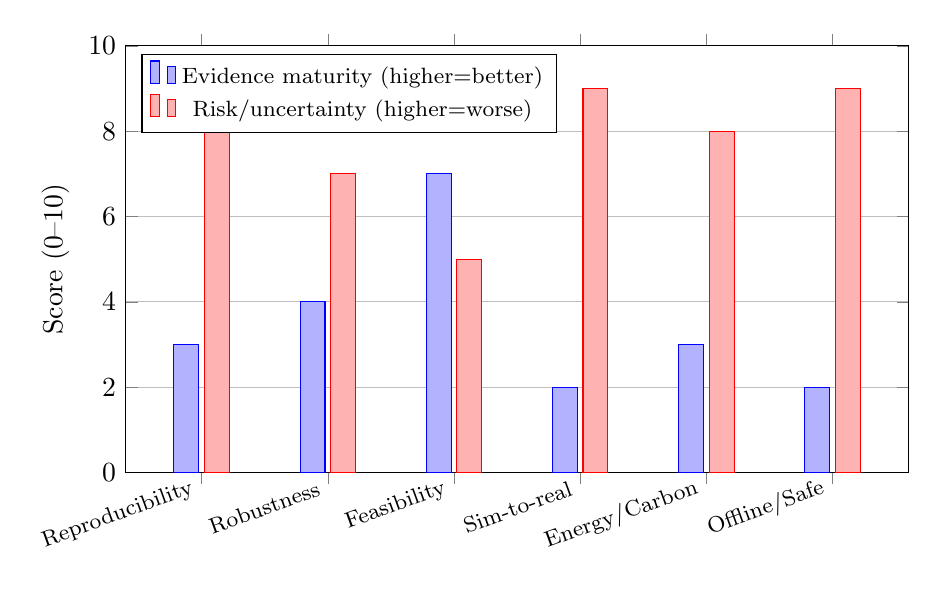
\begin{tikzpicture}
    \begin{axis}[
      width=0.95\linewidth,
      height=7cm,
      ybar,
      symbolic x coords={Reproducibility,Robustness,Feasibility,Sim-to-real,Energy/Carbon,Offline/Safe},
      xtick=data,
      ymin=0,ymax=10,
      ylabel={Score (0--10)},
      enlarge x limits=0.12,
      legend style={at={(0.02,0.98)}, anchor=north west, font=\footnotesize},
      ymajorgrids=true,
      bar width=9pt,
      xticklabel style={font=\footnotesize, rotate=20, anchor=east}
      ]
      \addplot coordinates {(Reproducibility,3) (Robustness,4) (Feasibility,7) (Sim-to-real,2) (Energy/Carbon,3) (Offline/Safe,2)};
      \addplot coordinates {(Reproducibility,8) (Robustness,7) (Feasibility,5) (Sim-to-real,9) (Energy/Carbon,8) (Offline/Safe,9)};
      \legend{Evidence maturity (higher=better),Risk/uncertainty (higher=worse)}
    \end{axis}
  \end{tikzpicture}
  \caption{Cross-cutting gaps in RL scheduling. Evidence maturity reflects how consistently studies report seeds, ablations, and real tests; risk captures brittleness and missing validation. Scores are qualitative and derived from the surveyed corpus.}
  \label{fig:crosscutting-gaps}
\end{figure}

\begin{figure}[t]\centering
  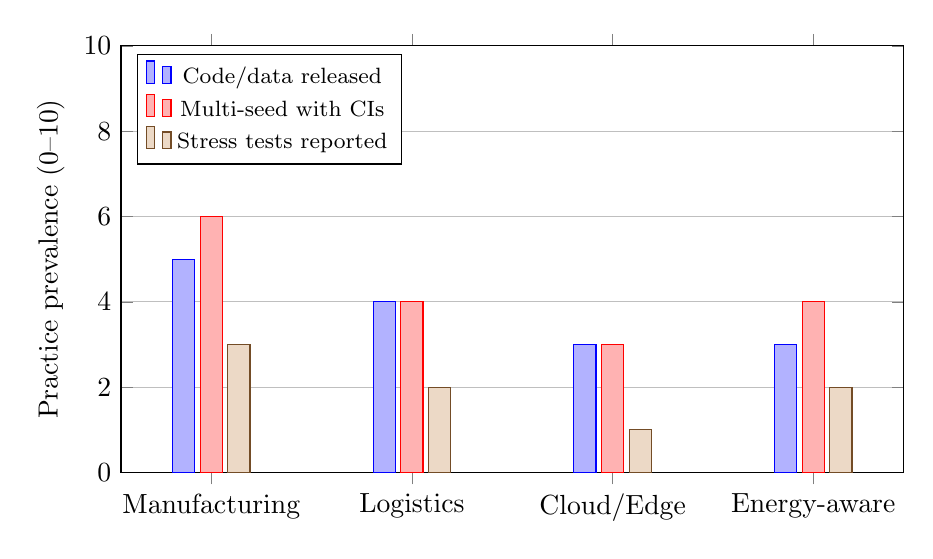
\begin{tikzpicture}
    \begin{axis}[
      width=0.95\linewidth,
      height=7cm,
      ybar,
      bar width=8pt,
      symbolic x coords={Manufacturing,Logistics,Cloud/Edge,Energy-aware},
      xtick=data,
      ymin=0,ymax=10,
      ylabel={Practice prevalence (0--10)},
      legend style={at={(0.02,0.98)}, anchor=north west, font=\footnotesize},
      ymajorgrids=true,
      enlarge x limits=0.15
      ]
      \addplot coordinates {(Manufacturing,5) (Logistics,4) (Cloud/Edge,3) (Energy-aware,3)};
      \addplot coordinates {(Manufacturing,6) (Logistics,4) (Cloud/Edge,3) (Energy-aware,4)};
      \addplot coordinates {(Manufacturing,3) (Logistics,2) (Cloud/Edge,1) (Energy-aware,2)};
      \legend{Code/data released,Multi-seed with CIs,Stress tests reported}
    \end{axis}
  \end{tikzpicture}
  \caption{Reporting practice prevalence across domains (qualitative scores from the surveyed corpus).}
  \label{fig:practice-coverage}
\end{figure}

\chapter{Open Gaps and Future Directions}
\label{c:future}
This chapter translates the observed gaps into a concise research agenda. Table~\ref{tab:future-roadmap} lays out short-, mid-, and long-term actions. Figure~\ref{fig:future-priority} maps priority against feasibility to highlight tractable wins versus moonshots.
\section{Hybrid RL and Operations Research}
Learning-augmented heuristics and primal-dual hybrids can turn RL signals into guided search rather than monolithic policies. RL-guided operator selection (memetic/EDA/GA) shows energy gains but needs controlled ablations against pure metaheuristics and exact MILP on small instances \cite{du2022_kbrl_fjsp}. Promising experiments include: (i) RL-warm starts for MILP/CP with primal-dual bounds; (ii) adaptive operator portfolios driven by learned critics; (iii) hybrid learners that swap between mask-driven feasibility and local search refinement.
Two concrete tracks can accelerate evidence: (1) \textbf{Operator ablations}: fix problem seeds and compare GA/EDA/NSGA-II with and without RL-guided operator choice, matching compute budgets and reporting runtime-quality Pareto curves. (2) \textbf{Primal-dual warm starts}: feed MILP/CP with RL-suggested partial schedules and measure bound tightening and solve time. Both require logging exact solver gaps and making code reproducible. Runtime overhead and complexity of integration (CPLEX/Gurobi hooks) should be reported.
Hybrid pipelines should also explore \textbf{anytime} behavior: measure solution quality over time and contrast against purely heuristic baselines. For dynamic settings, hybrid repairers that trigger on constraint violations (or predicted violations) can serve as shields with better quality than simple vetoes. Finally, incorporating uncertainty sets (interval processing times, arrival ranges) into hybrids may yield more robust schedules than point estimates.
\section{Offline, Safe, and Risk-Sensitive RL}
Offline RL and behavior cloning can exploit historic shop-floor and cloud logs, reducing simulator dependence \cite{mauro2023_offline}. BCQ/CRR/CQL baselines should accompany online agents, with safety constraints enforced via shields or Lyapunov critics for feasibility-sensitive shops \cite{gottwald2021_safe}. Practical next steps: build logged datasets with action/constraint traces; evaluate shielded offline agents; report safety KPIs (violations/hour) alongside makespan.
An actionable recipe: (i) collect or release logs with states, actions, masks, constraints, and outcomes; (ii) train BCQ/CRR/CQL with and without mask-aware critics; (iii) deploy shielded offline policies in shadow mode; (iv) compare to online fine-tuning starting from offline checkpoints. Report degradation under distribution shift (new product mix, new cloud traces) and the value of conservative Q-learning for safety. Risk-sensitive objectives (CVaR, chance constraints) should be experimented with for dynamic, safety-critical shops; even small toy MILP instances with exact feasibility checks can anchor these claims.
Safe RL research should quantify latency overhead of shields and vetoes, and measure how often shields fire in practice. Pairing shields with uncertainty estimation (ensembles, dropout) can lower override frequency while maintaining safety. Publishing shield logic and test harnesses (unit tests for infeasible actions) will make safety claims auditable.
\section{Transfer, Meta-Learning, and Continual Adaptation}
Meta-RL and size-generalizable policies (e.g., YOTO) hint at “train once, reuse often” for dynamic shops \cite{zeng2022_yoto_jss, tong2023_meta}. Future work should test cross-factory transfer, curriculum over tariffs and disturbances, and continual learning with replay buffers that protect against catastrophic forgetting. Standardized environments such as TransferJSS remain a key enabler \cite{tassel2020_transferjss}.
Concrete experiments: (i) train on FT/Taillard small/medium, test on LA/hybrid instances; (ii) curriculum over price signals and disturbance patterns (arrivals, downtime); (iii) continual evaluation where product mix shifts gradually, measuring retention vs.\ forgetting; (iv) meta-RL across domains (manufacturing $\rightarrow$ logistics) to test representation reuse. Reporting should include adaptation speed (episodes to recover), final gap vs.\ from-scratch training, and whether policies respect unseen constraints after transfer.
For cloud/edge, cross-trace generalization (provider A trace $\rightarrow$ provider B), and edge-device churn tests (nodes joining/leaving) would mirror real deployment. For logistics, layout changes (aisle reconfiguration) and demand shifts are the analogues. Continual learning safeguards (replay with diversity, elastic weight consolidation) should be benchmarked for scheduling, not just robotic control.
\section{Benchmarking and Standardization}
Progress depends on transparent, repeatable benchmarks: fixed train/val/test splits across instance sizes; disturbance scenarios for dynamic/online settings; tariff/emission sweep protocols for energy-aware work. Reporting should include gap-to-optimum where MILP/CP is feasible, win-rate vs.\ strong metaheuristics, seed sensitivity, and release of code/data (checklist in Table~\ref{tab:repro-checklist}).
To make progress cumulative, three artifacts are needed: (1) \textbf{Benchmark blueprints} with public instance generators, disturbance/tariff catalogs, and evaluation scripts; (2) \textbf{Baseline suites} (Table~\ref{tab:baseline-suite}) with tuned heuristics/metaheuristics and exact solvers where feasible; (3) \textbf{Metric packs} that include feasibility rates, safety KPIs, runtime, and carbon/energy units where relevant. Table~\ref{tab:benchmark-blueprint} sketches such a blueprint. Community challenges (yearly leaderboards) could anchor reproducibility by requiring code submission and reruns on held-out splits.
Standardized log formats (states, actions, masks, constraints, rewards, timestamps) would unlock offline RL benchmarks akin to D4RL but for scheduling. Lightweight digital twins could provide deterministic and stochastic modes for consistent evaluation. Finally, agreement on reporting seeds and confidence intervals is low-hanging fruit; papers lacking this should be considered incomplete.

\section{Deployment and Pilot Playbooks}
Closing the loop from simulation to production requires explicit pilot plans. A staged playbook includes: (i) offline replay on historical logs; (ii) shadow mode with veto-only actions; (iii) limited-scope actuation with human override; (iv) gradual scale-up with A/B comparisons against heuristics. Table~\ref{tab:pilot-plan} outlines a minimal pilot checklist. Each stage should log overrides, violations, runtime, and operator feedback.
\section{Data, Carbon, and Compute Accountability}
Future work should track data provenance (which factory/trace, which time window), carbon/energy impact of training and inference, and fairness of comparisons. Including training/inference energy (kWh) and carbon estimates alongside scheduler energy objectives avoids shifting cost from runtime to training. Compute-efficient baselines (small transformers/MLPs vs.\ large GNNs) should be compared for cost-benefit. For cloud/edge, PUE/thermal constraints ought to be part of the environment, not post-hoc.

\begin{table}[t]\centering\small
  \caption{Roadmap for advancing RL scheduling research.}
  \label{tab:future-roadmap}
  \begin{tabular}{p{2.1cm}p{3.2cm}p{5.4cm}p{3.5cm}}
\hline
\textbf{Horizon} & \textbf{Goal} & \textbf{Key tasks} & \textbf{Dependencies/Deliverables} \\
\hline
Short-term (0--6 mo) & Make studies reproducible and fair & Release code/data or generators; multi-seed runs with CIs; mask/shield ablations; tariff/emission sweeps for energy-aware cases; report gap-to-optimum where MILP fits & Checklists (Table~\ref{tab:repro-checklist}); updated baselines; public splits \\
\hline
Mid-term (6--18 mo) & Strengthen robustness and offline safety & Build logged datasets; add BCQ/CRR/CQL baselines; evaluate shielded policies; disturbance/domain-randomized tests (arrivals, processing noise, tariffs) & Open log-based benchmarks; robustness reports with stress suites \\
\hline
Mid-term (6--18 mo) & Hybrid RL+OR that beats tuned metaheuristics & RL-guided operator portfolios; primal-dual warm starts; compare to GA/NSGA-II/EDA and MILP/CP on small instances; runtime vs.\ quality analysis & Reproducible hybrid pipelines; ablation reports; runtime/quality Pareto plots \\
\hline
Long-term (18+ mo) & Generalizable, safe, sim-to-real schedulers & Cross-plant/trace transfer; continual/meta-RL; sim-to-real pilots for yards/shops; interpretable dashboards with overrides & Multi-domain benchmark suite (manufacturing, logistics, cloud); pilot reports with safety KPIs \\
\hline
\end{tabular}

\end{table}

\begin{figure}[t]\centering
  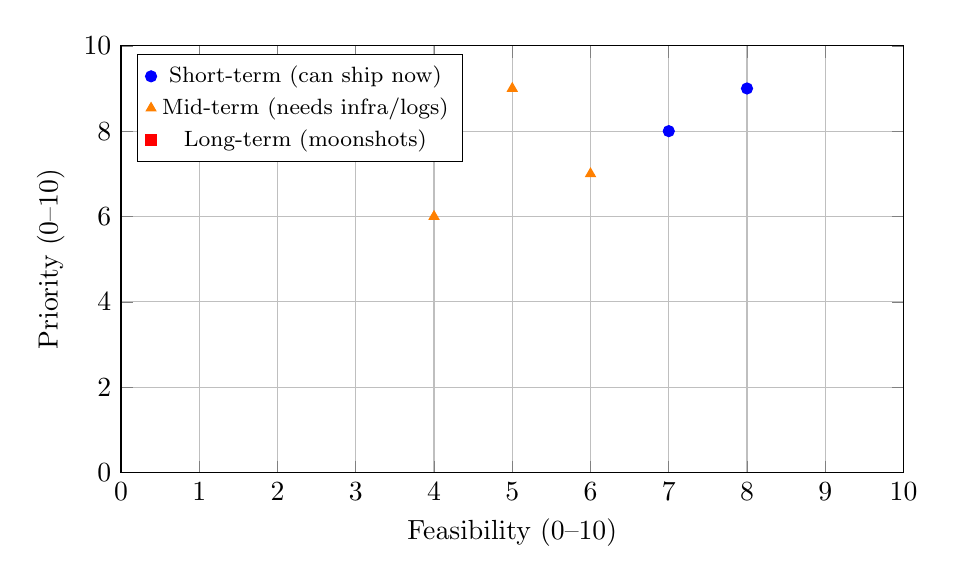
\begin{tikzpicture}
    \begin{axis}[
      width=0.95\linewidth,
      height=7cm,
      xlabel={Feasibility (0--10)},
      ylabel={Priority (0--10)},
      xmin=0,xmax=10,ymin=0,ymax=10,
      grid=both,
      legend style={at={(0.02,0.98)}, anchor=north west, font=\footnotesize},
      scatter/classes={
        short={mark=*,blue},
        mid={mark=triangle*,orange},
        long={mark=square*,red}
      }
    ]
    \addplot[scatter,only marks,scatter src=explicit symbolic]
      coordinates {
        (8,9) [short]
        (7,8) [short]
        (6,7) [mid]
        (5,9) [mid]
        (4,6) [mid]
        (3,8) [long]
        (2,9) [long]
      };
    \addlegendimage{scatter,only marks,mark=*,blue}
    \addlegendentry{Short-term (can ship now)}
    \addlegendimage{scatter,only marks,mark=triangle*,orange}
    \addlegendentry{Mid-term (needs infra/logs)}
    \addlegendimage{scatter,only marks,mark=square*,red}
    \addlegendentry{Long-term (moonshots)}
    \end{axis}
  \end{tikzpicture}
  \caption{Priority vs.\ feasibility for proposed directions. Short-term focuses on reproducibility, masking/shield ablations, and tariff sweeps; mid-term targets offline RL on logs and hybrid RL+OR ablations; long-term spans sim-to-real pilots and standardized multi-domain benchmarks.}
  \label{fig:future-priority}
\end{figure}

\begin{table}[t]\centering\small
  \caption{Blueprint for a reusable multi-domain benchmark pack.}
  \label{tab:benchmark-blueprint}
  \begin{tabular}{p{2.9cm}p{3.8cm}p{3.8cm}p{4cm}}
\hline
\textbf{Domain} & \textbf{Instances/traces} & \textbf{Disturbances/tariffs} & \textbf{Eval metrics and scripts} \\
\hline
Manufacturing (JSS/FJSS) & FT/LA/Taillard train/val/test splits; mixed routing depths; blocking/no-wait variants & Arrival bursts; setup variability; machine downtime; TOU/RTP tariffs (energy/carbon) & Makespan/tardiness; feasibility rate; energy/carbon cost; runtime; gap-to-optimum (small) \\
\hline
Logistics/transport (AGV/yard/rail) & Open warehouse/yard layouts; metro corridor with timetable data & Blocked aisles; communication loss; demand surges; pad/headway constraints & Turnaround/delay; collisions/headway violations; override count; energy \\
\hline
Cloud/edge & Public traces (Google/Alibaba); DAG workflows; VM/rack topology & Workload shifts; bursty arrivals; network jitter; power caps; thermal throttling & Slowdown/latency (P95); SLA violations; energy; feasibility of actions; runtime \\
\hline
Energy/carbon-aware (cross-domain) & Tariff catalogs (flat/TOU/RTP); emission factors; paired with above instances & Tariff/emission sweeps; demand charges; DR events & kWh, kg CO$_2$e, energy cost vs throughput; Pareto fronts; sensitivity plots \\
\hline
\end{tabular}

\end{table}

\begin{table}[t]\centering\small
  \caption{Pilot deployment checklist for RL schedulers.}
  \label{tab:pilot-plan}
  \begin{tabular}{p{3cm}p{5cm}p{5cm}}
\hline
\textbf{Stage} & \textbf{Actions} & \textbf{Artifacts/KPIs} \\
\hline
Offline replay & Train/evaluate on historical logs; add offline RL baselines; mask/shield unit tests & Violation/override counts (simulated); gap vs heuristics; runtime; seed CIs \\
\hline
Shadow mode & Run policy in parallel, no actuation; log suggested actions vs executed & Feasibility; latency; delta-to-heuristic KPIs; operator feedback; override frequency (simulated) \\
\hline
Limited actuation & Actuate on subset (machines/lanes/VMs) with human override; shields on & Real violation rate; time-to-safe-state; throughput/latency; energy/carbon; override count \\
\hline
Scale-up/A/B & Expand coverage; A/B test vs baseline heuristics/metaheuristics & Win-rate; KPI deltas; safety events; latency distribution; compute cost; confidence intervals \\
\hline
Postmortem and iterate & Analyze failures, overrides, safety events; refine masks/shields/rewards & Lessons log; updated configs; retraining cost; decision to promote/rollback \\
\hline
\end{tabular}

\end{table}

\begin{figure}[t]\centering
  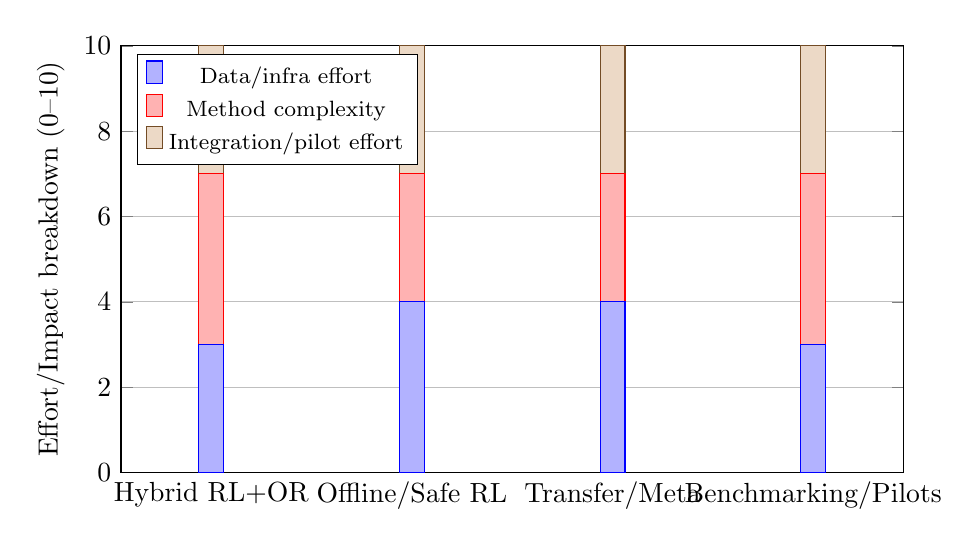
\begin{tikzpicture}
    \begin{axis}[
      width=0.95\linewidth,
      height=7cm,
      ybar stacked,
      bar width=9pt,
      symbolic x coords={Hybrid RL+OR,Offline/Safe RL,Transfer/Meta,Benchmarking/Pilots},
      xtick=data,
      ymin=0,ymax=10,
      ylabel={Effort/Impact breakdown (0--10)},
      legend style={at={(0.02,0.98)}, anchor=north west, font=\footnotesize},
      ymajorgrids=true,
      enlarge x limits=0.15
      ]
      \addplot coordinates {(Hybrid RL+OR,3) (Offline/Safe RL,4) (Transfer/Meta,4) (Benchmarking/Pilots,3)};
      \addplot coordinates {(Hybrid RL+OR,4) (Offline/Safe RL,3) (Transfer/Meta,3) (Benchmarking/Pilots,4)};
      \addplot coordinates {(Hybrid RL+OR,3) (Offline/Safe RL,3) (Transfer/Meta,3) (Benchmarking/Pilots,3)};
      \legend{Data/infra effort,Method complexity,Integration/pilot effort}
    \end{axis}
  \end{tikzpicture}
  \caption{Effort components for major research directions (qualitative stacks). Use to scope projects against available data, method maturity, and deployment appetite.}
  \label{fig:effort-stacks}
\end{figure}

\chapter{Conclusion}
\label{c:conclusion}
This thesis reviewed reinforcement learning for scheduling across manufacturing, logistics, cloud/edge, and energy-aware settings. RL policies now reliably beat dispatching rules and often narrow the gap to metaheuristics when feasibility masks and graph encoders are used; energy-aware hybrids show meaningful savings. However, reproducibility, robustness, and sim-to-real validation remain weak. The recommended path forward is to pair mask-based actors with strong baselines and multi-seed reporting, integrate offline/safe RL with shields for feasibility-critical plants, and adopt standardized benchmarks with tariff/disturbance sweeps. Closing these gaps will determine whether RL schedulers move from promising simulators to dependable production tools.

\section*{Current state of evidence}
Across domains, feasibility-preserving designs (masks, eligibility checks) are the backbone of competitive RL schedulers. Graph encoders and attention sharpen performance and generalization for JSS/FJSS, while lightweight state vectors suffice for cloud/edge when paired with robust baselines. Energy-aware hybrids show consistent energy/carbon reductions with small throughput trade-offs. Yet, most evidence is simulator-bound, often single-seed, and light on stress tests. Logistics and cloud work remain largely unvalidated on hardware; manufacturing studies seldom report gap-to-optimum or runtime vs.\ heuristics. Reproducibility is uneven, with only a handful of open codebases and public traces.

\section*{Actionable next steps by domain}
\textbf{Manufacturing/semiconductor} — Publish code and mask logic; report gap-to-optimum on small instances; include setup/downtime disturbances; test tariff sensitivity for energy-aware variants; shadow deploy with veto-only mode before any actuation. \\
\textbf{Logistics/transport} — Add disturbance suites (blocked aisles, comms loss), headway/collision metrics, and latency budgets; incorporate demand forecasting for repositioning; pursue shielded MARL for safety-critical rail/pad constraints; pilot on logs with Real2Sim-style randomization. \\
\textbf{Cloud/edge} — Use public traces; report slowdown CIs, SLA violation curves, and decision latency; add bin-packing + DVFS baselines; model network jitter and churn; include power/thermal caps in the environment. \\
\textbf{Energy/carbon-aware} — Sweep tariffs (flat/TOU/RTP) and emission factors; report absolute units (kWh, kg CO$_2$e) and Pareto fronts; explore demand charges/DR events; couple production and transport emissions where relevant.

\section*{Research agenda in brief}
Four themes summarize the way forward. First, \textbf{feasibility-first design}: masks, shields, and interpretable overrides must be non-negotiable for any deployment. Second, \textbf{evidence discipline}: multi-seed runs with confidence intervals, strong baselines, and stress tests should become table stakes. Third, \textbf{hybridization and reuse}: RL should warm-start or guide OR/search, and offline/meta-RL should reuse logs to cut sample demands. Fourth, \textbf{sim-to-real pathways}: standardized benchmarks, tariff/disturbance catalogs, and staged pilots (shadow$\rightarrow$limited$\rightarrow$scale) are needed before real-world actuation. Delivering on these themes will turn today’s promising experimental results into trustworthy schedulers that operators can adopt with confidence.

\section*{Operational playbook for deployment}
1) \textbf{Offline replay}: validate on historical logs with mask/shield tests and offline RL baselines. \\
2) \textbf{Shadow mode}: run in parallel, no actuation; log deltas vs.\ heuristics, feasibility, latency, and overrides. \\
3) \textbf{Limited actuation}: start small (subset of machines/lanes/VMs) with human override, shields on; monitor safety KPIs and runtime. \\
4) \textbf{A/B and scale}: compare against tuned heuristics/metaheuristics; report CIs, violations, and energy/carbon where relevant; rollback triggers defined. \\
5) \textbf{Postmortem}: publish failures, overrides, and fixes; update masks/shields and retrain; re-run stress suites.

\section*{Final outlook}
RL-driven scheduling has crossed the threshold of reliably outperforming classic dispatching rules and often rivals hand-tuned metaheuristics, especially in dynamic and energy-aware settings. The bottlenecks are no longer solely algorithmic—they are about evidence, safety, and trust. A disciplined pipeline that combines mask-based feasibility, multi-seed reporting, strong baselines, offline and hybrid methods, and staged pilots will decide whether RL schedulers stay in papers or end up on shop floors, in yards, and in data centers. With transparent benchmarks and deployment playbooks, the field can move from promising demos to dependable, auditable scheduling systems.
